\section{Introduction}

For this report we evaluate the capabilities of texture-features extracted with the Leung-Malik (LM) filter bank of finding images similar to a given one. In the following sections we will extract descriptors based on texture filters and then use a knn-search algorithm to retrieve the most fitting images.

\section{Leung-Malik Filter Bank}

We use the Matlab code provided by the Visual Geometry Group of Oxford University to create the LM filter bank\footnote{\url{http://www.robots.ox.ac.uk/\~vgg/research/texclass/filters.html}}. The bank consists of 48 different filters at different scales and orientations: 36 first and second derivatives of Gaussians at 6 different orientations and 3 scales, 8 Laplacian of Gaussian (LOG) filters, and 4 Gaussian filters. Figure \ref{fig:lmFilter} shows the filters visualized as heat maps.

\begin{figure}[!hbt]
  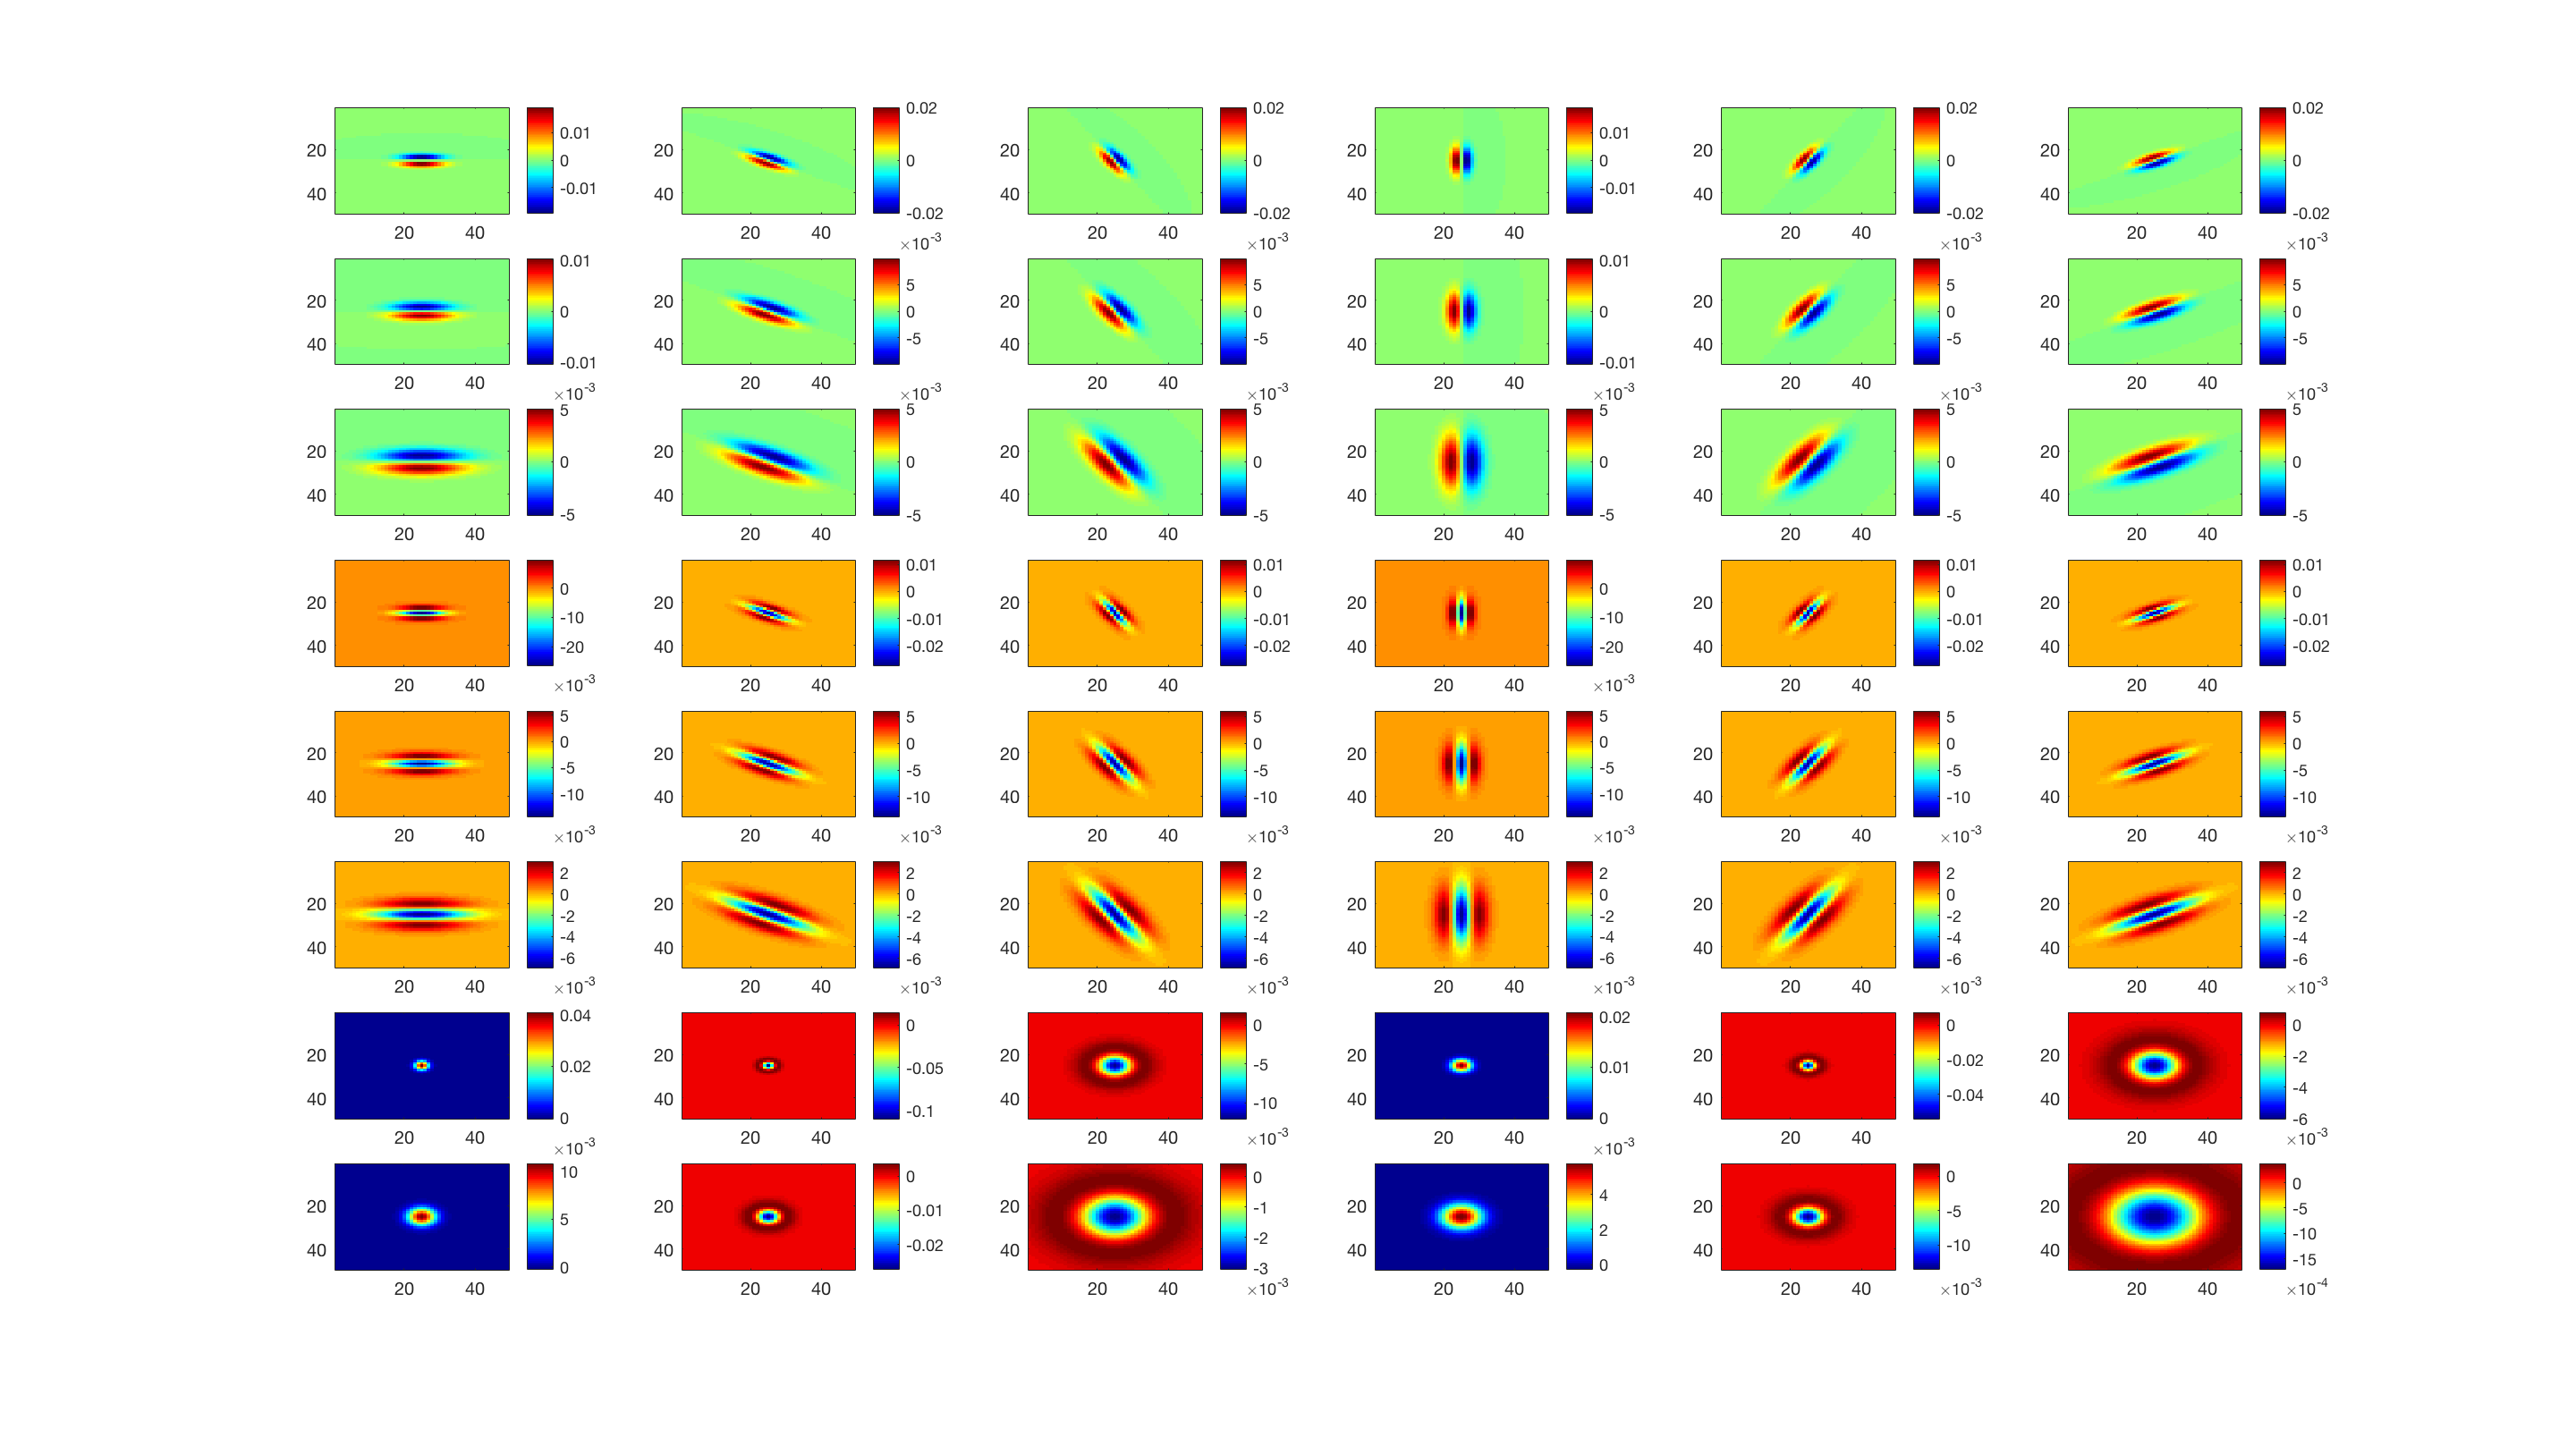
\includegraphics[width=\textwidth]{img/LM_filter_bank}
  \caption{Visualization of LM filter bank}
  \label{fig:lmFilter}
\end{figure}


\section{Texture Descriptors}

\begin{figure}[!hbt]
\centering
\subfigure[Example image \texttt{forest\_9}]{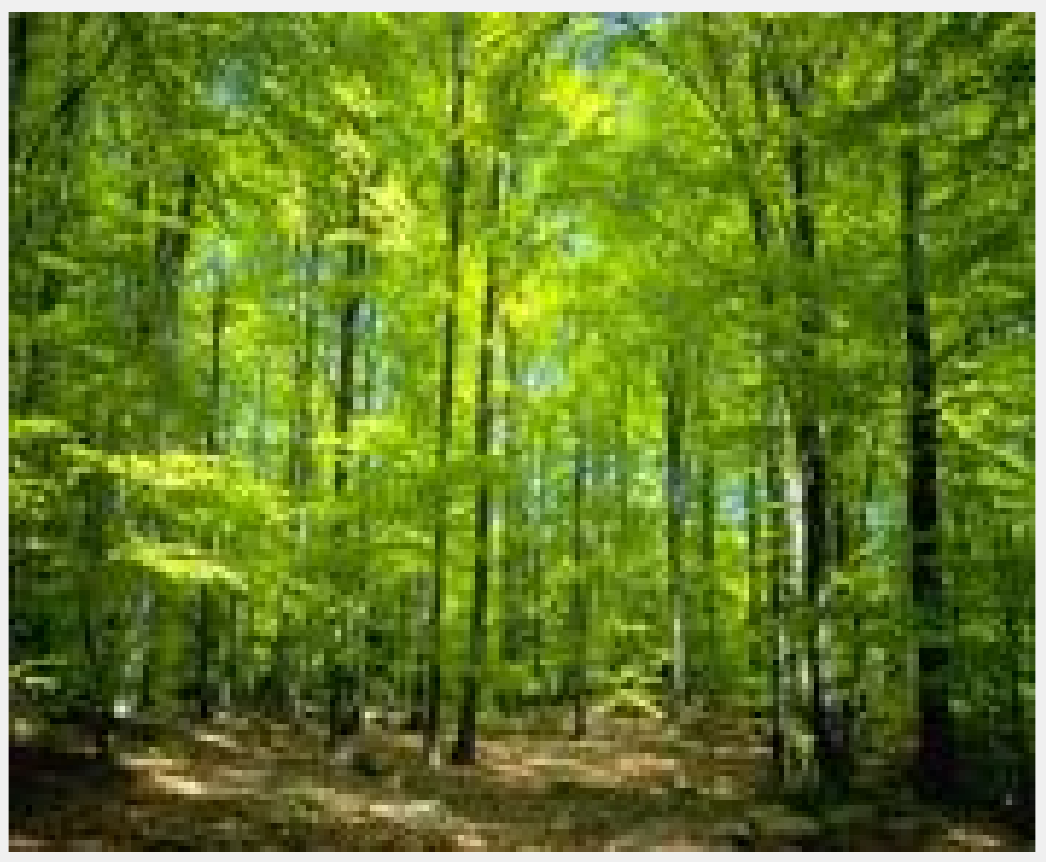
\includegraphics[width=0.4\textwidth]{img/f9}} \\
\subfigure[Responses of \texttt{forest\_9} to the LM filter bank]{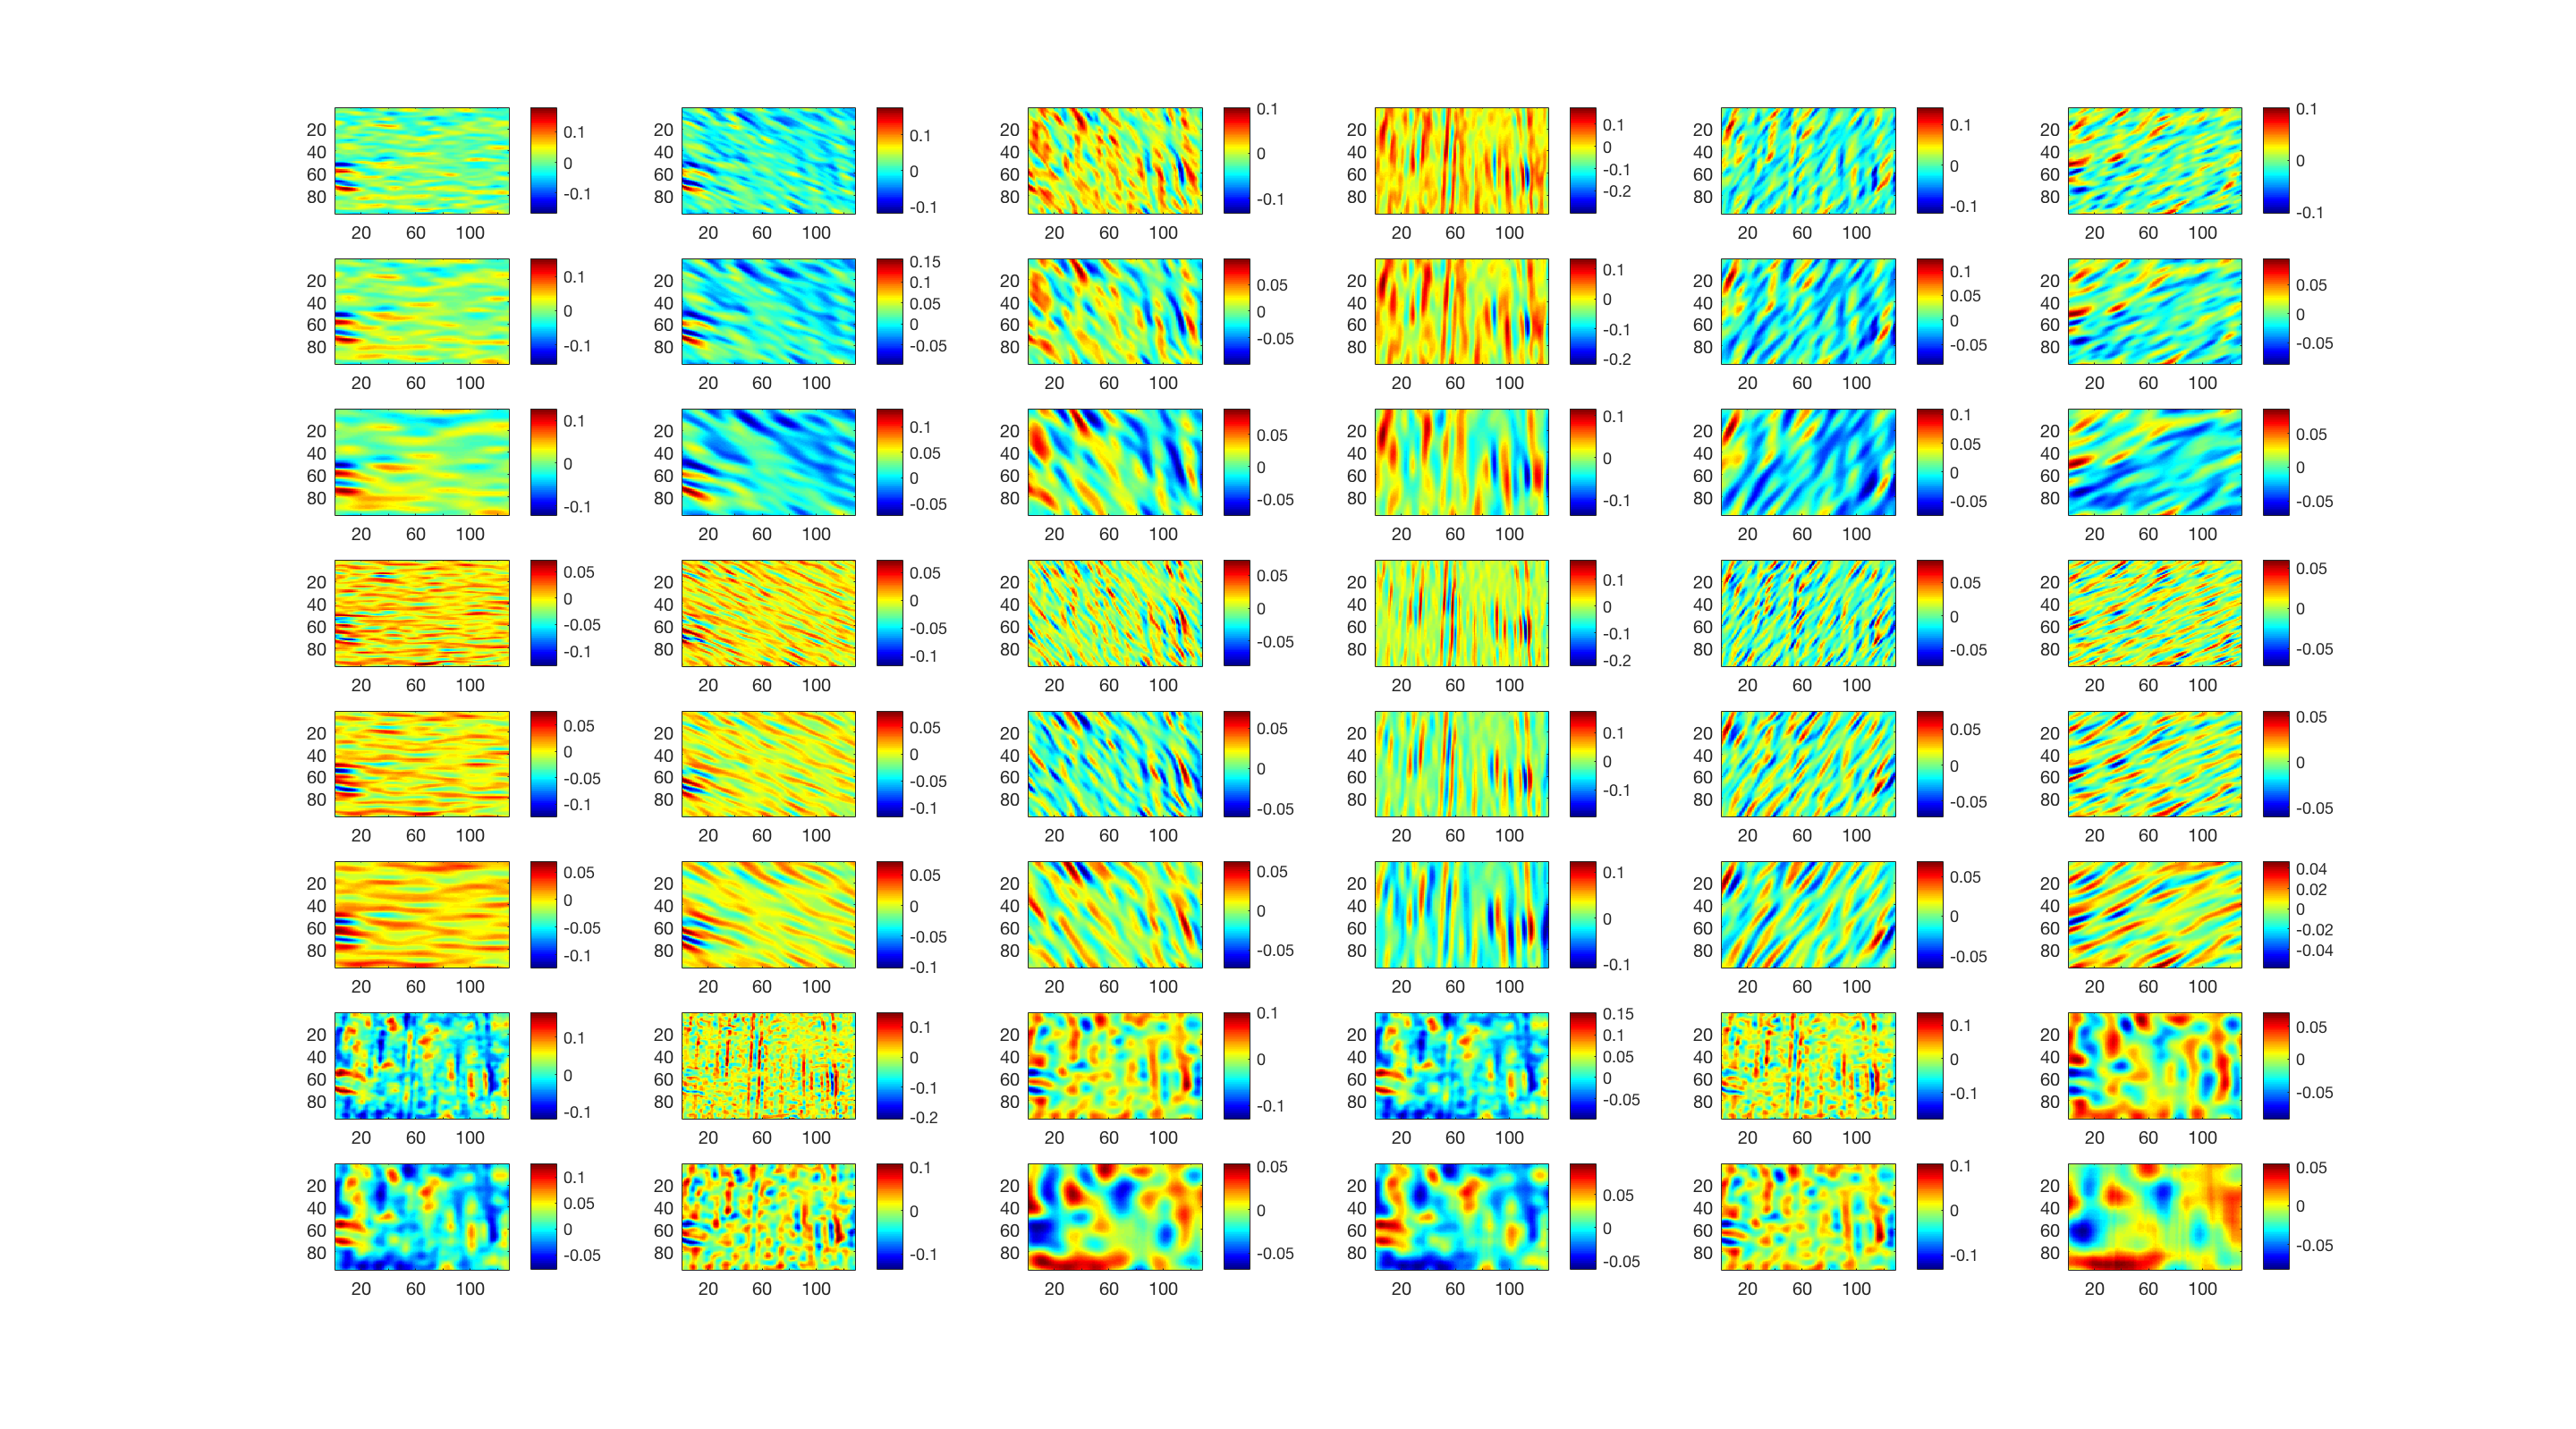
\includegraphics[width=0.9\textwidth]{img/f9_responses}} \\
\subfigure[Normalized responses of \texttt{buildings\_2} to the LM filter bank. The heat map colors are relative to the global minimum (-0.2982) and maximum (0.1799) of responses for this particular image.]{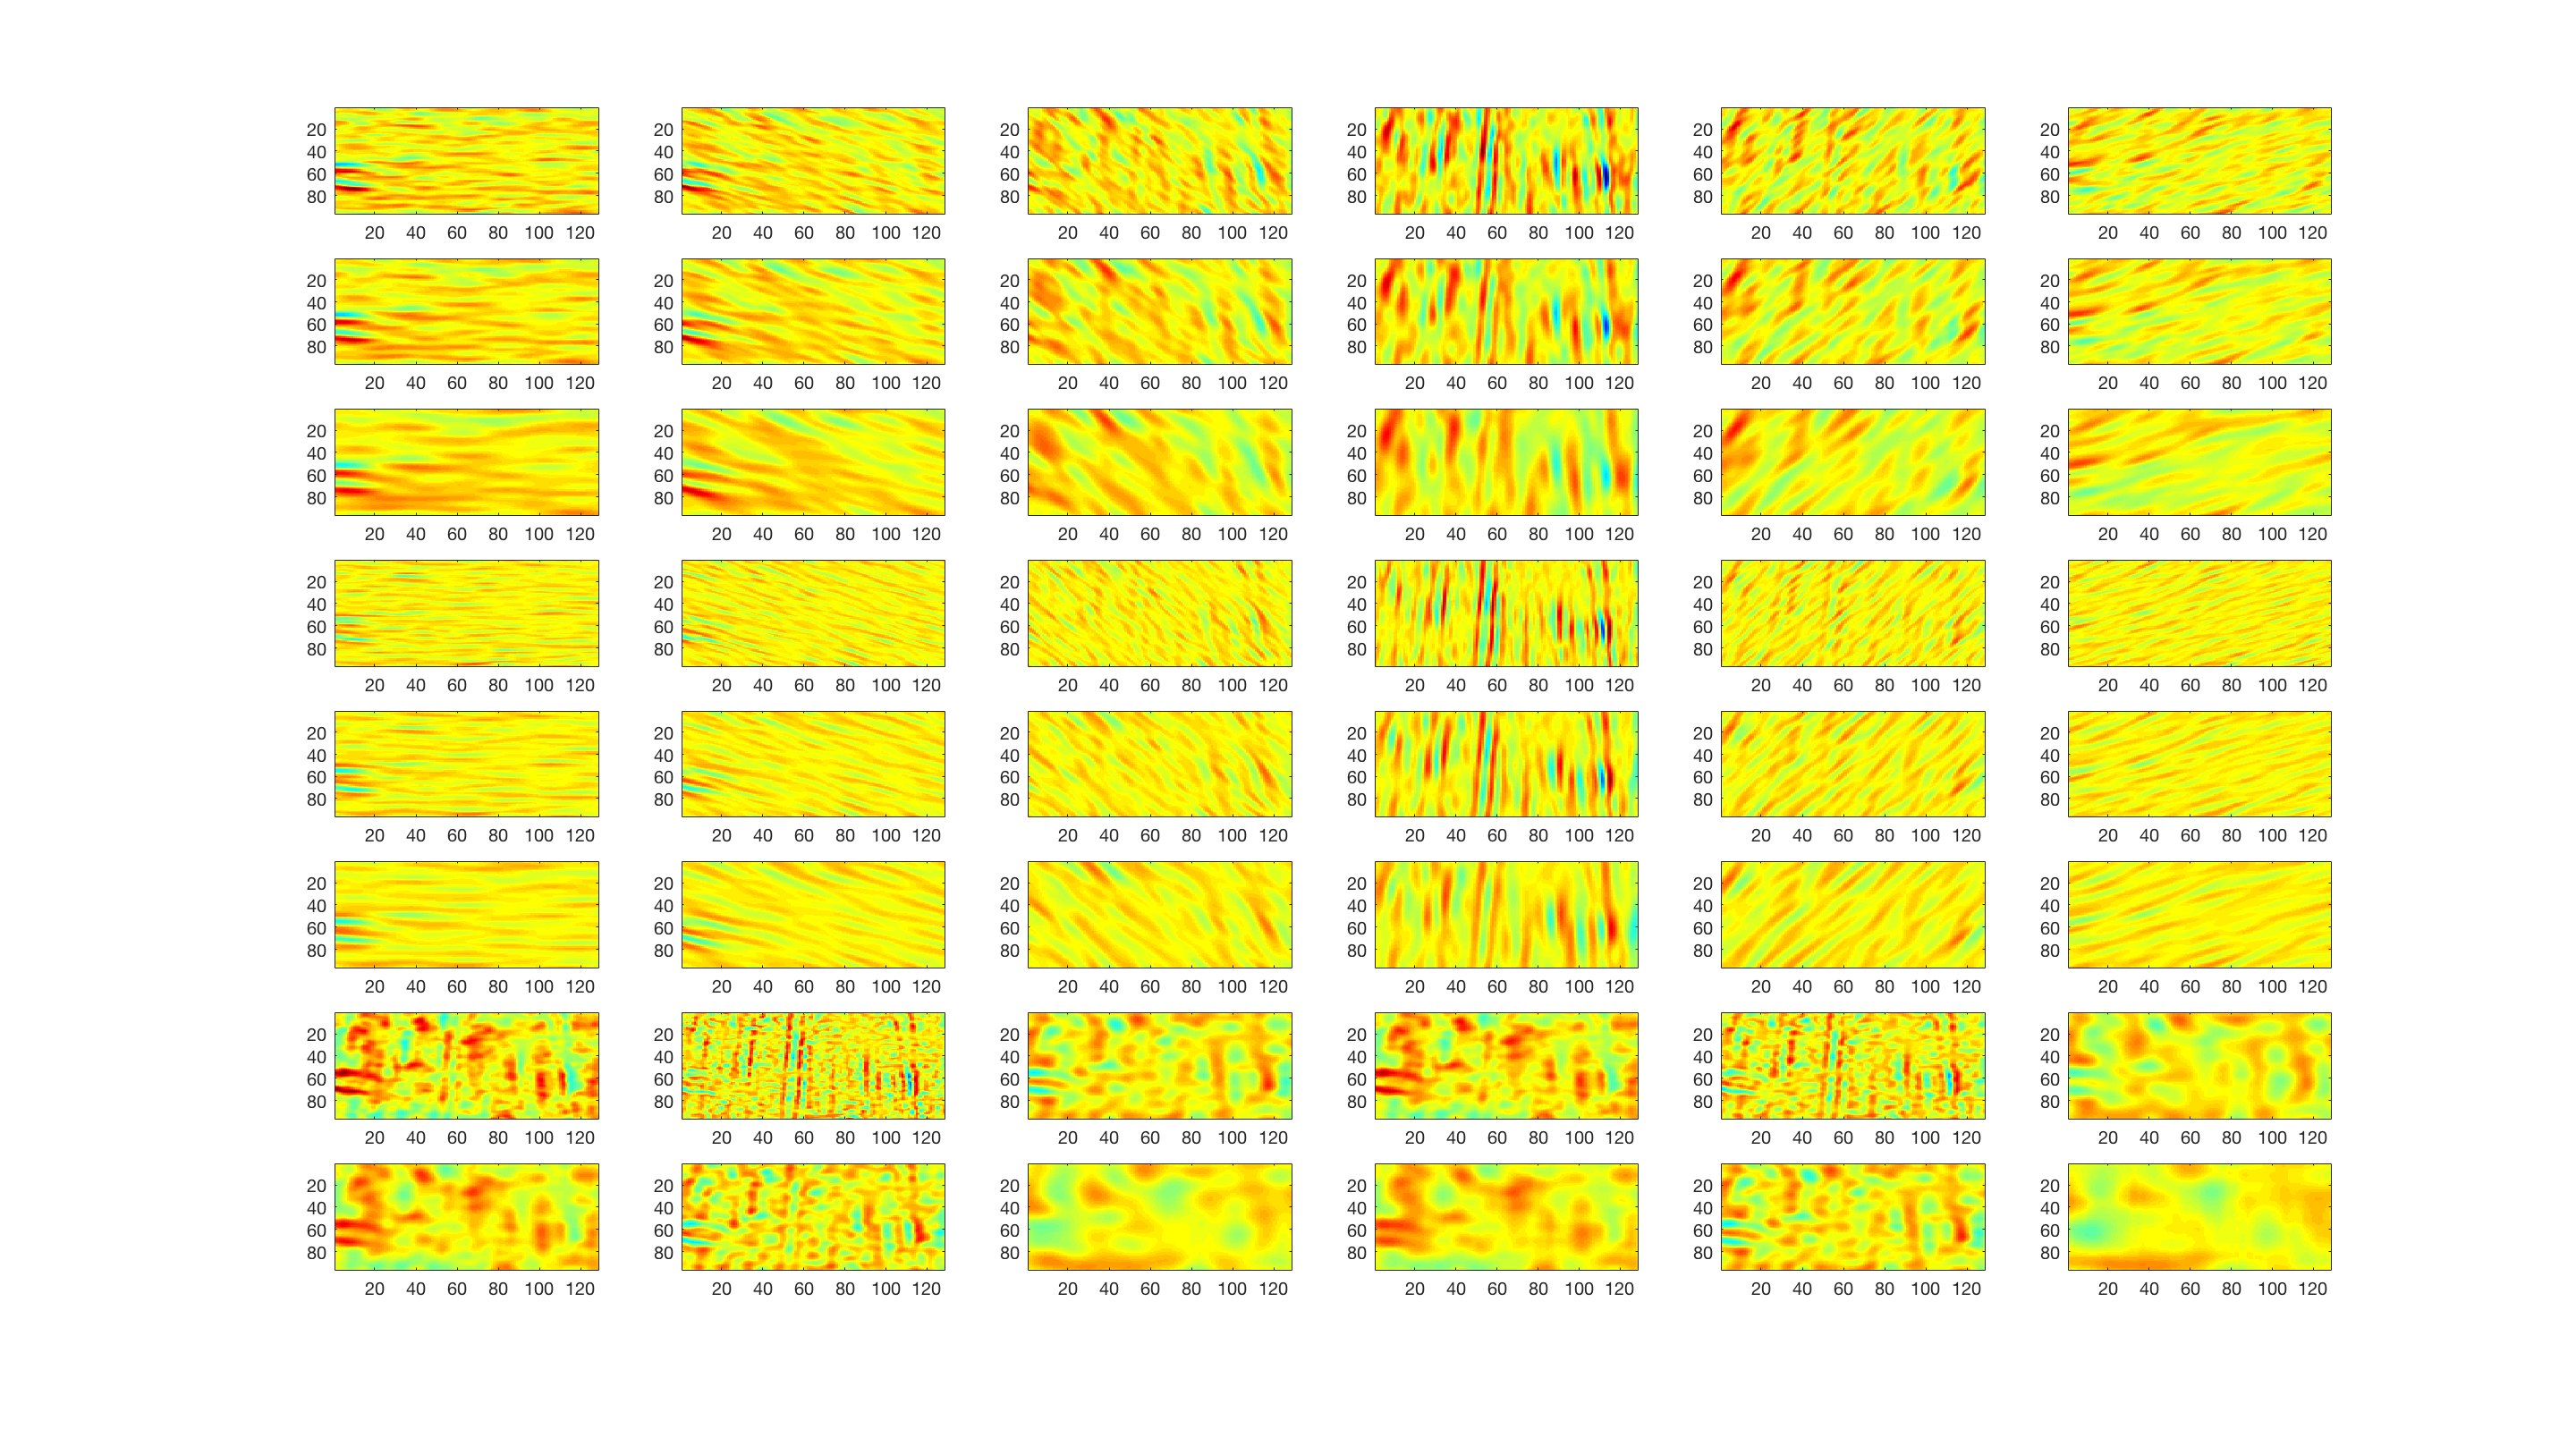
\includegraphics[width=0.9\textwidth]{img/f9_responses_normalized}}
\caption{Visualization of the LM filter bank responses applied on a forest image}
\label{fig:f9Response}
\end{figure}

\begin{figure}[!hbt]
\centering
\subfigure[Example image \texttt{buildings\_2}]{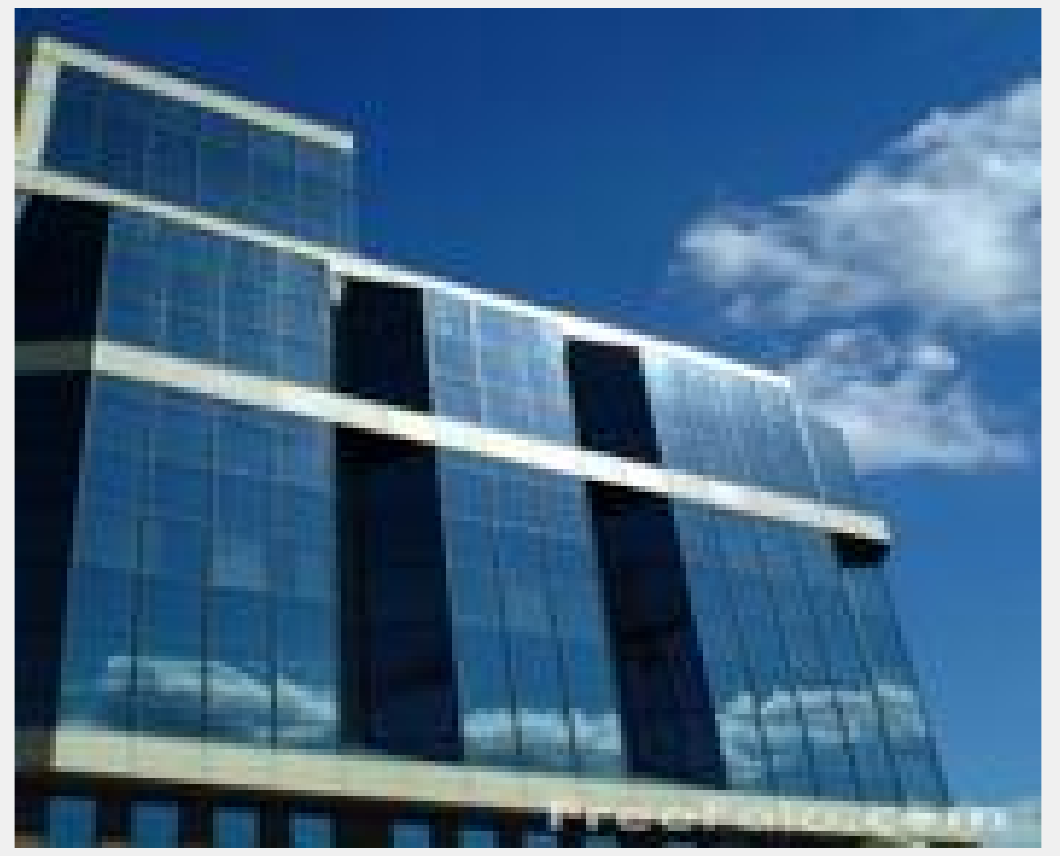
\includegraphics[width=0.4\textwidth]{img/b2}} \\
\subfigure[Normalized responses of \texttt{buildings\_2} to the LM filter bank. The heat map colors are relative to the global minimum (-0.3498) and maximum (0.3828) of responses for this particular image.]{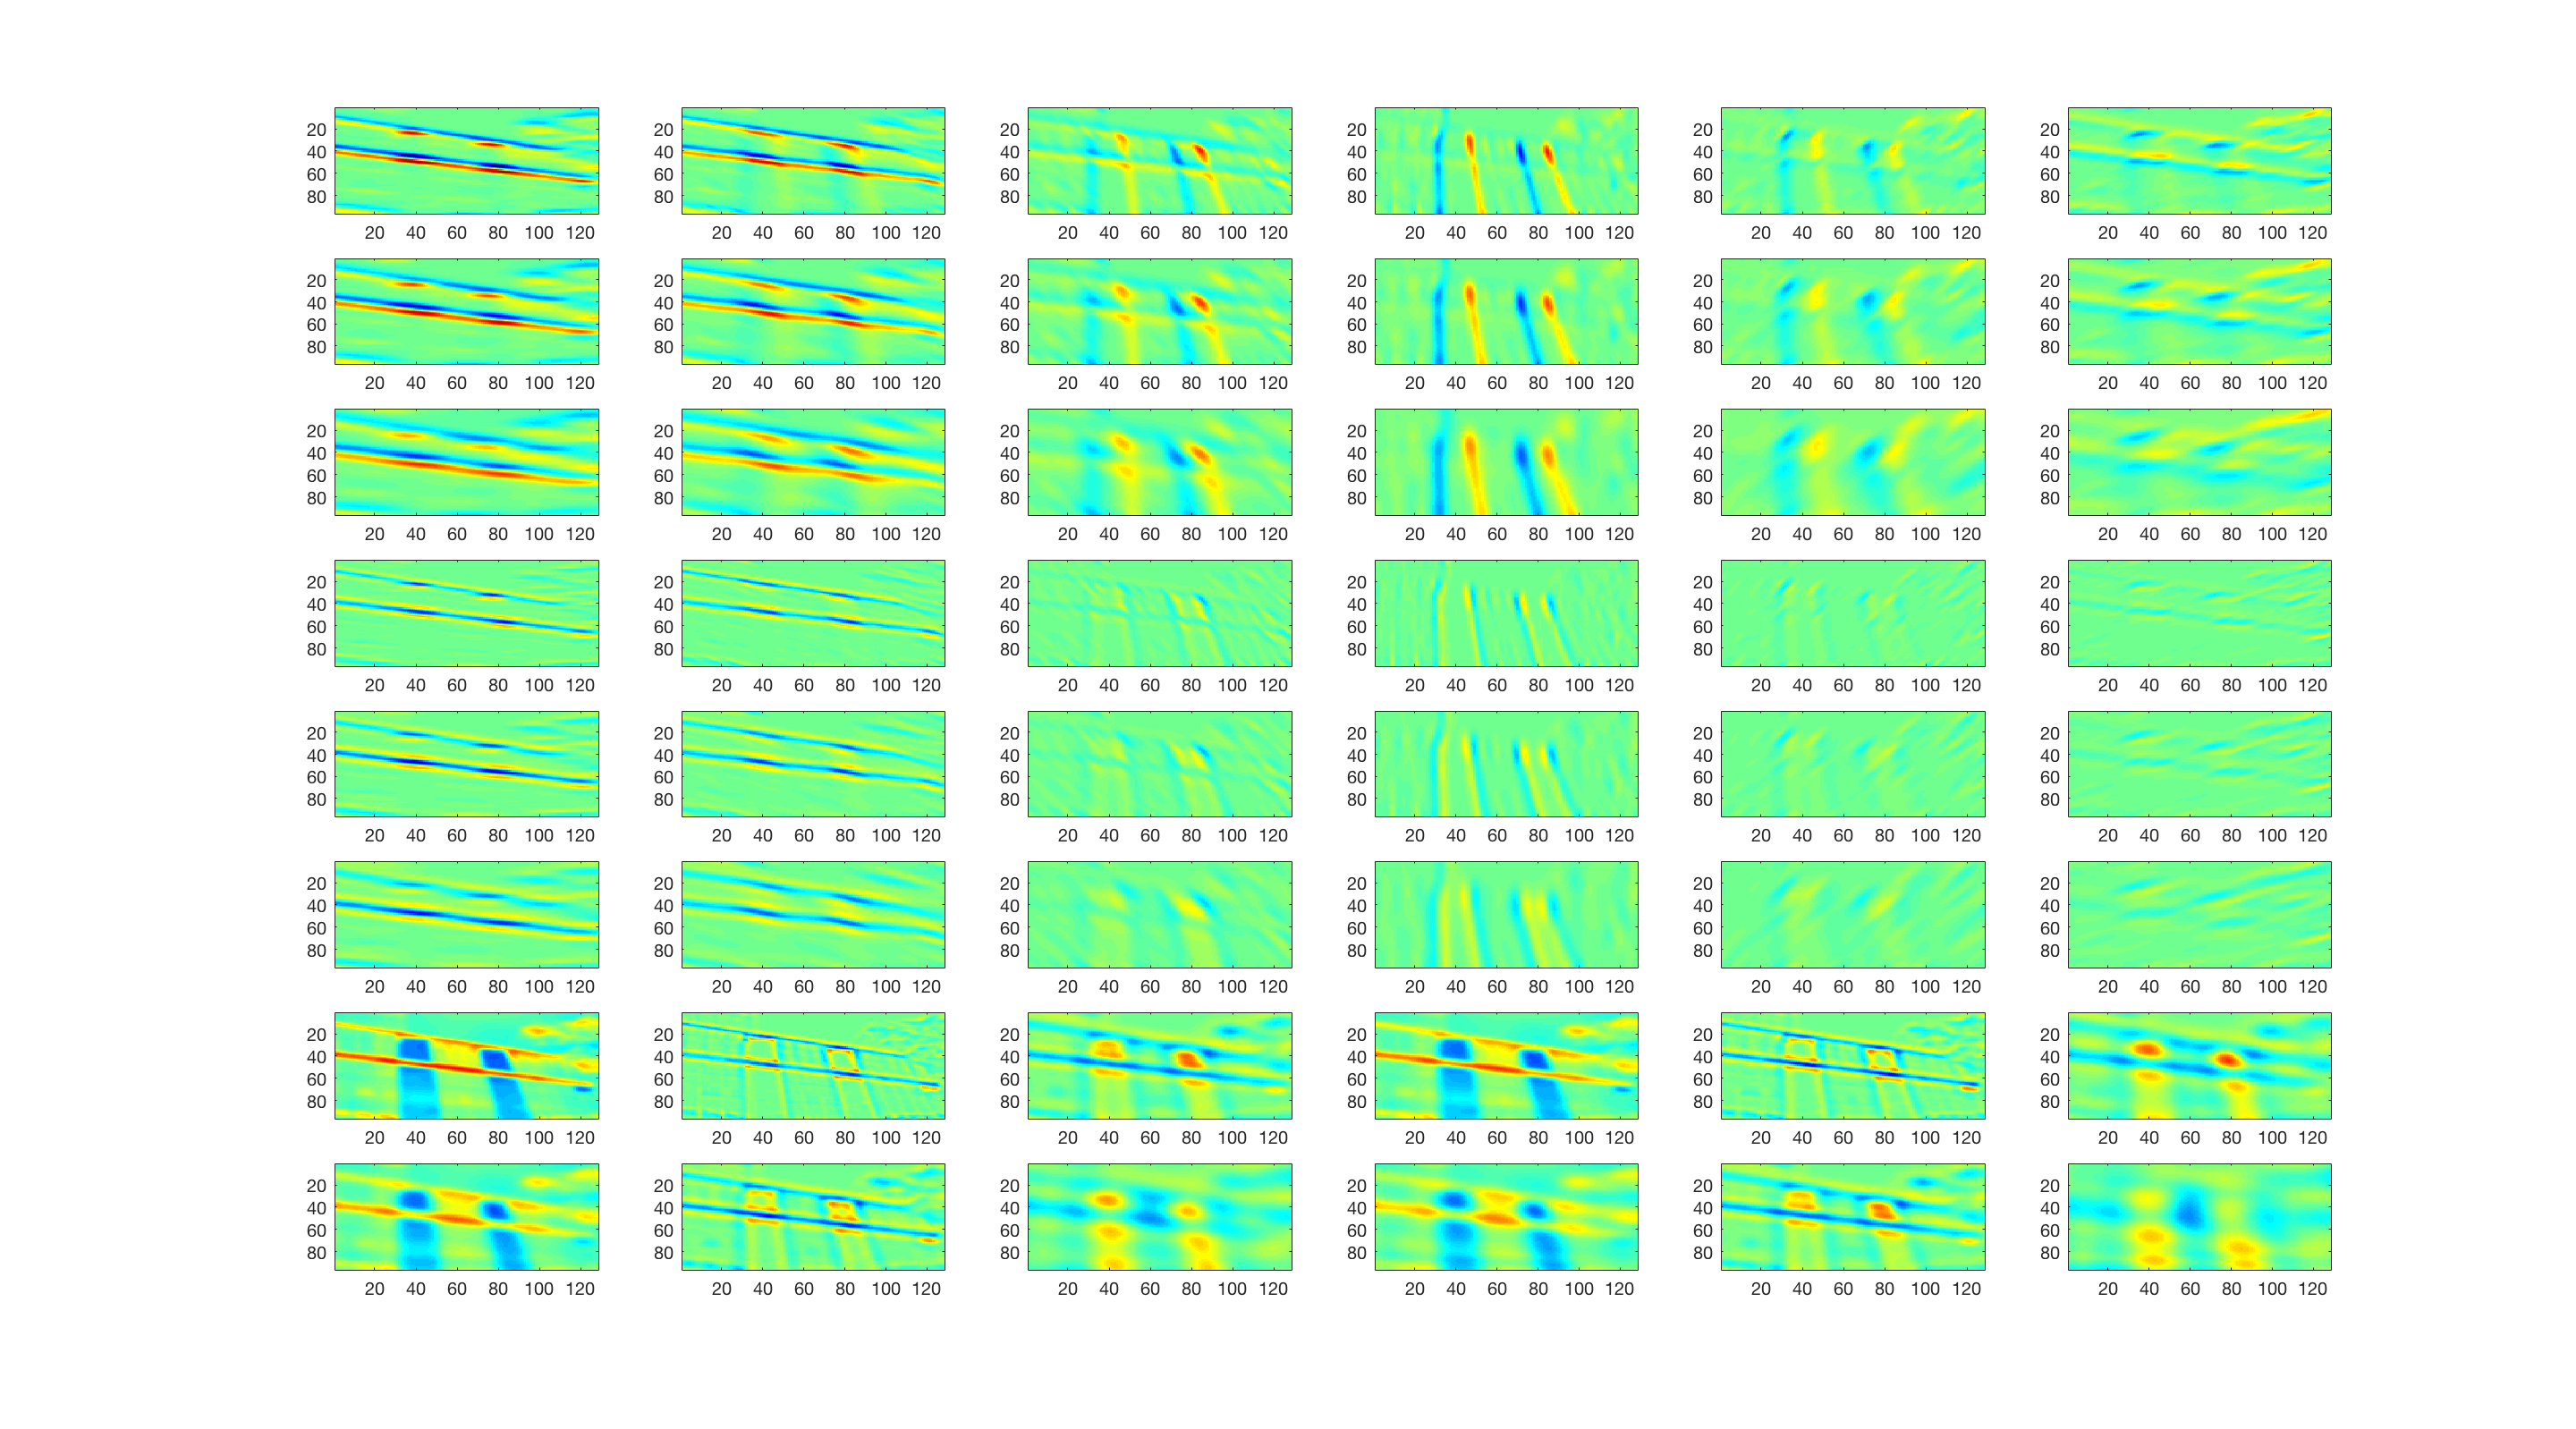
\includegraphics[width=0.9\textwidth]{img/b2_responses_normalized}}
\caption{Visualization of the LM filter bank responses applied on a buildings image}
\label{fig:b2Response}
\end{figure}


\begin{figure}[!hbt]
\centering
\subfigure[test]{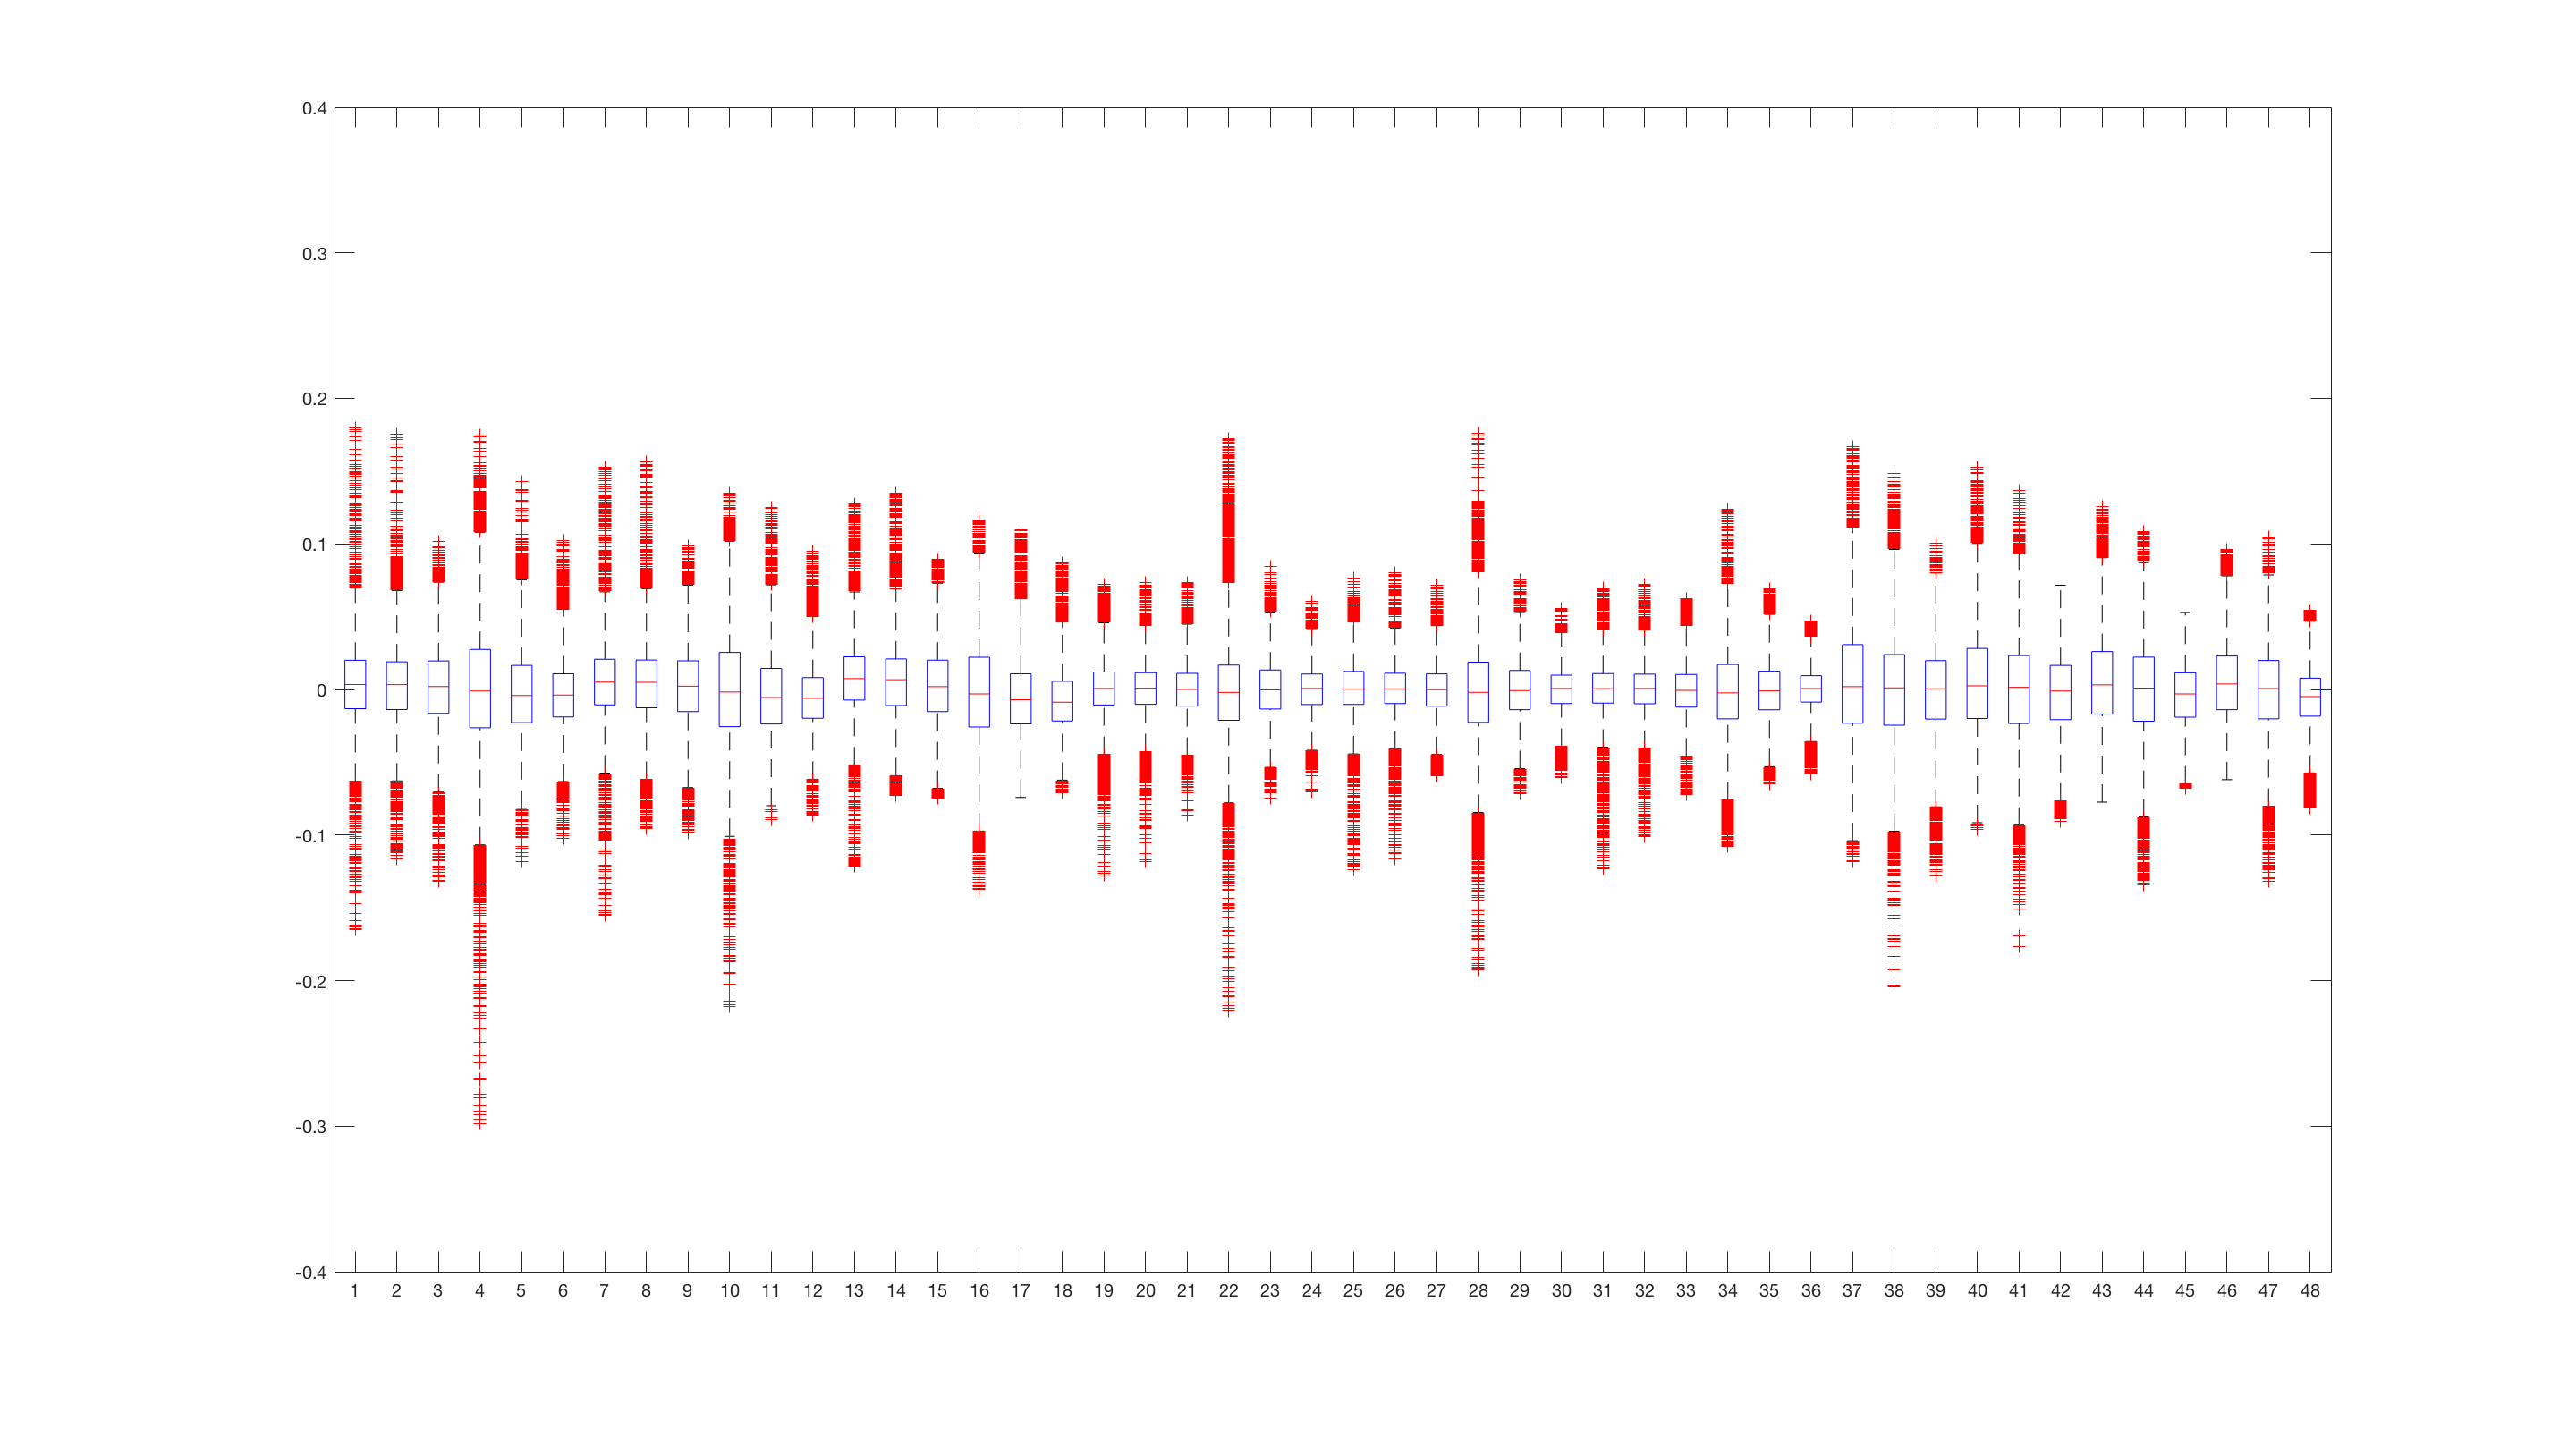
\includegraphics[width=\textwidth]{img/f9_boxplots}} \\
\subfigure[test]{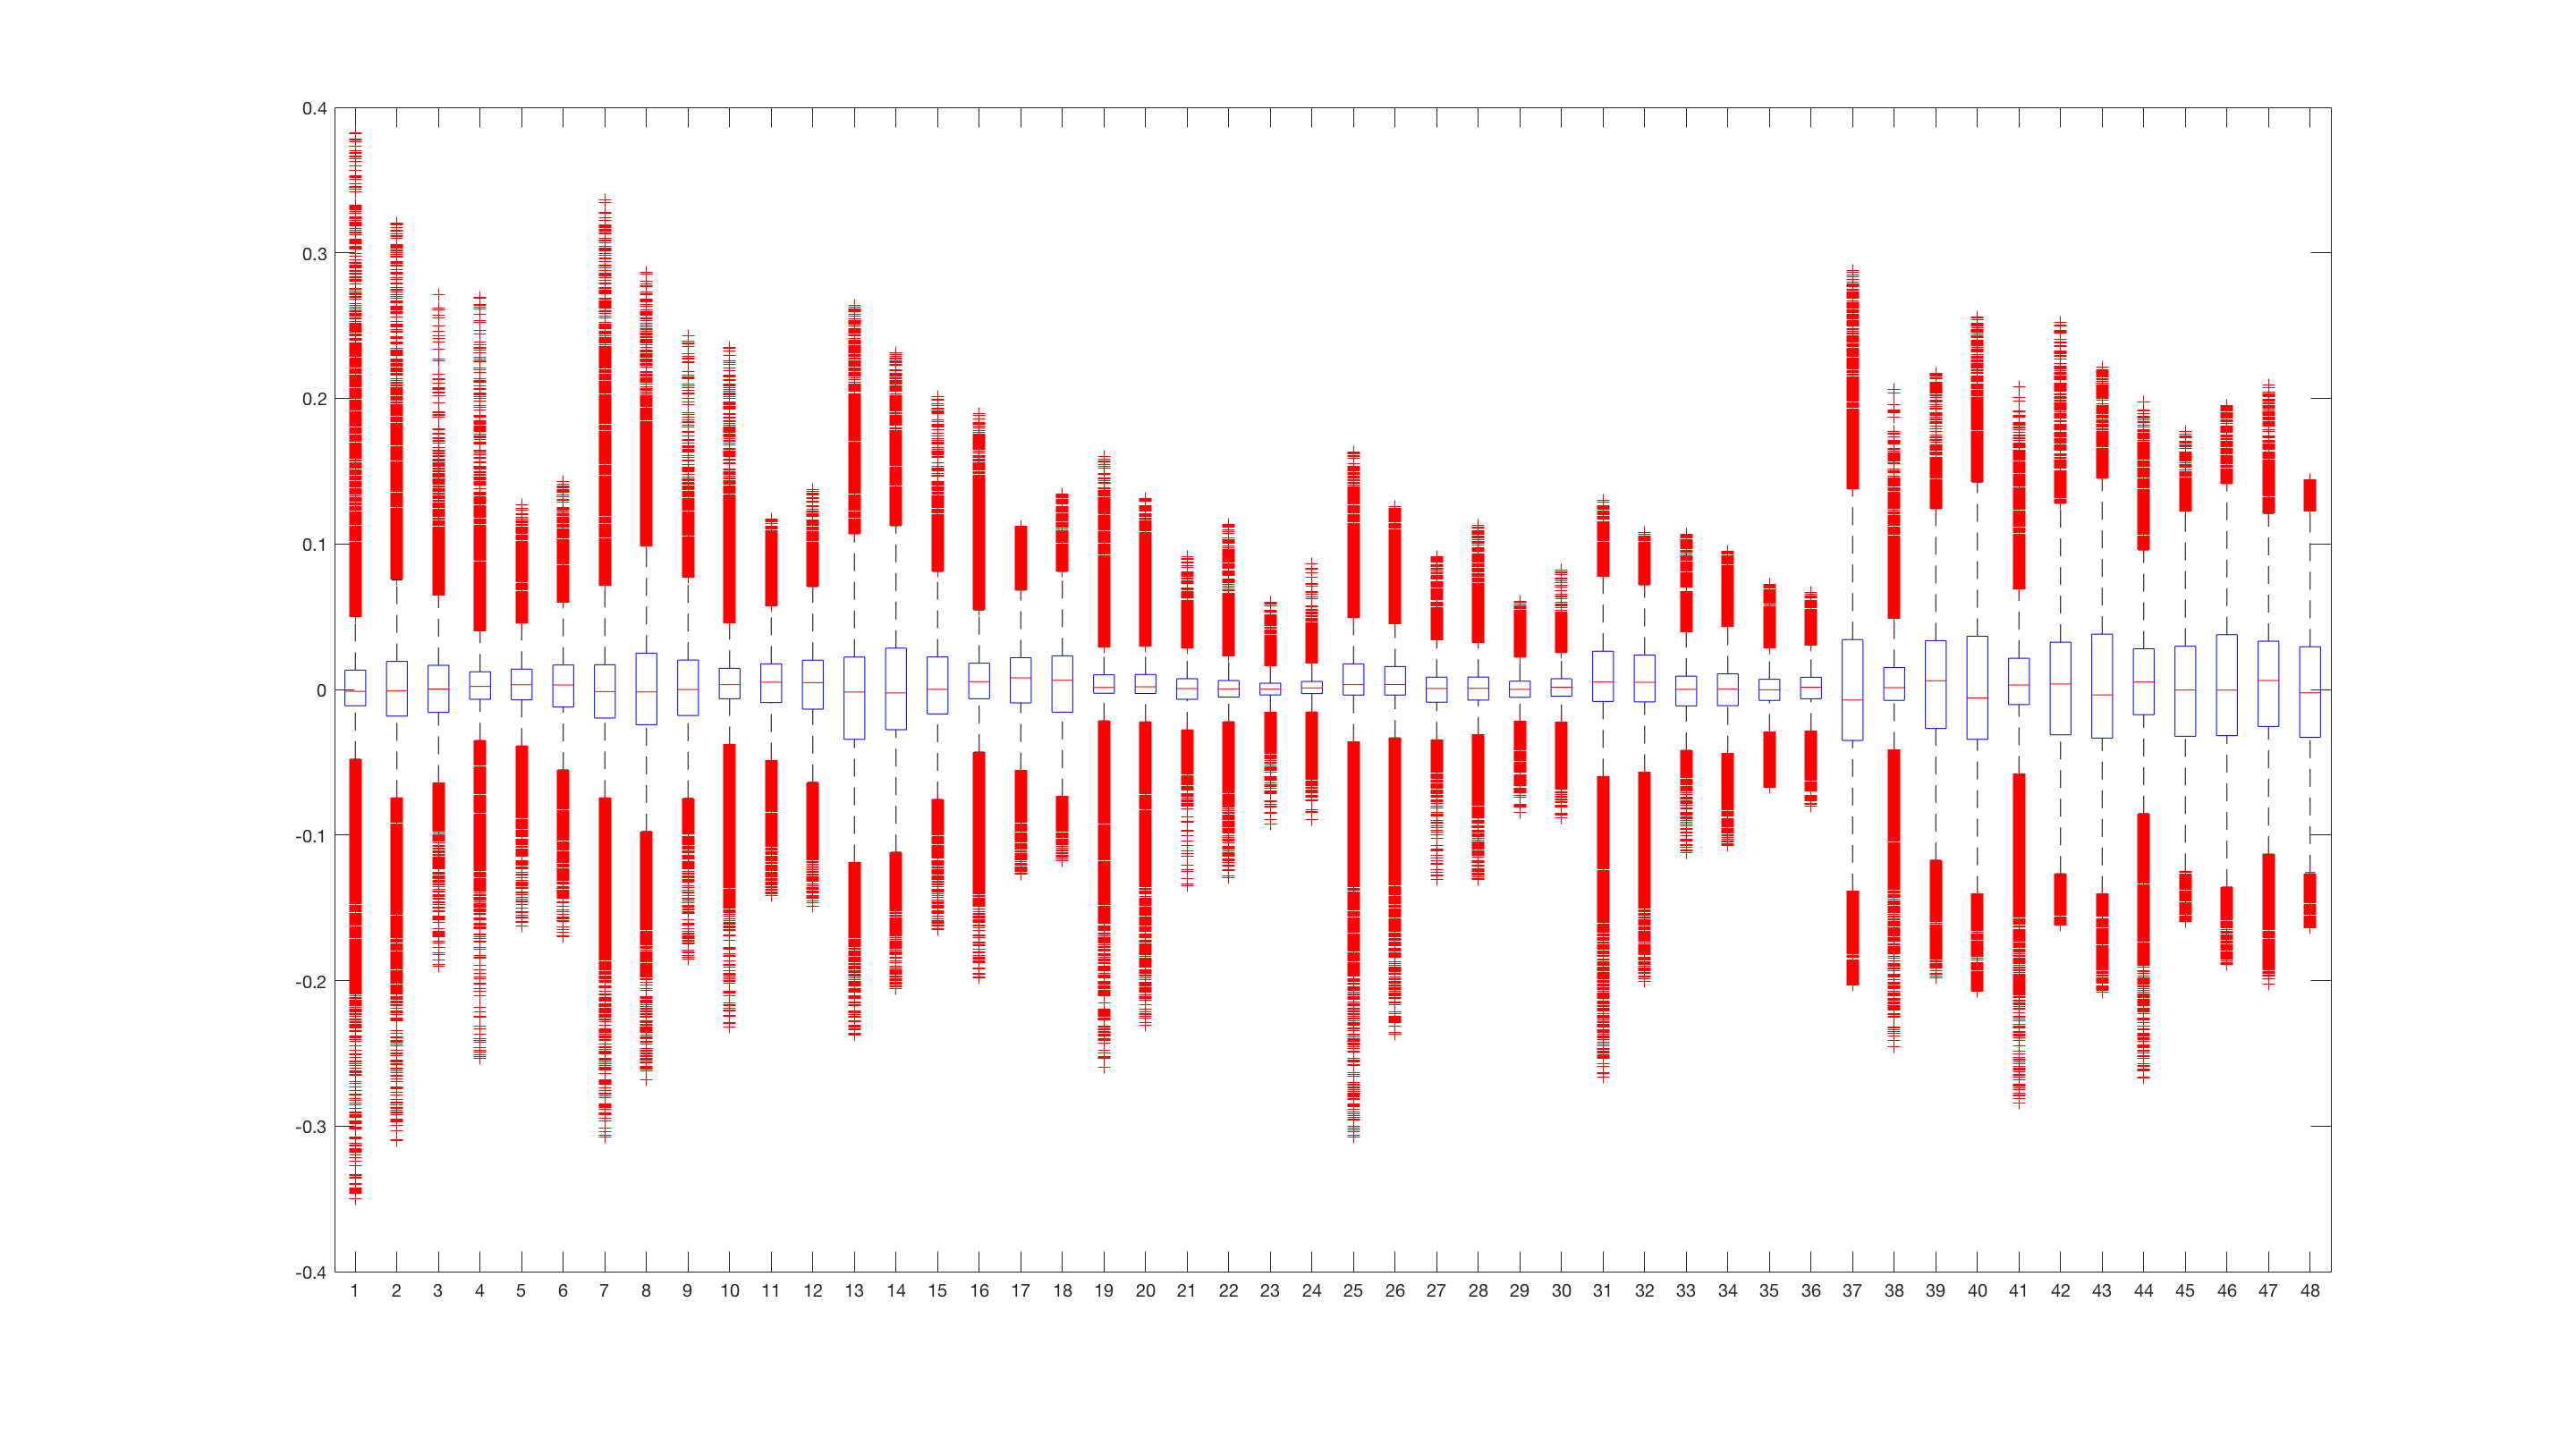
\includegraphics[width=\textwidth]{img/b2_boxplots}}
\caption{cap}
\label{fig:boxplots}
\end{figure}


\begin{figure}[!hbt]
\centering
\subfigure[test]{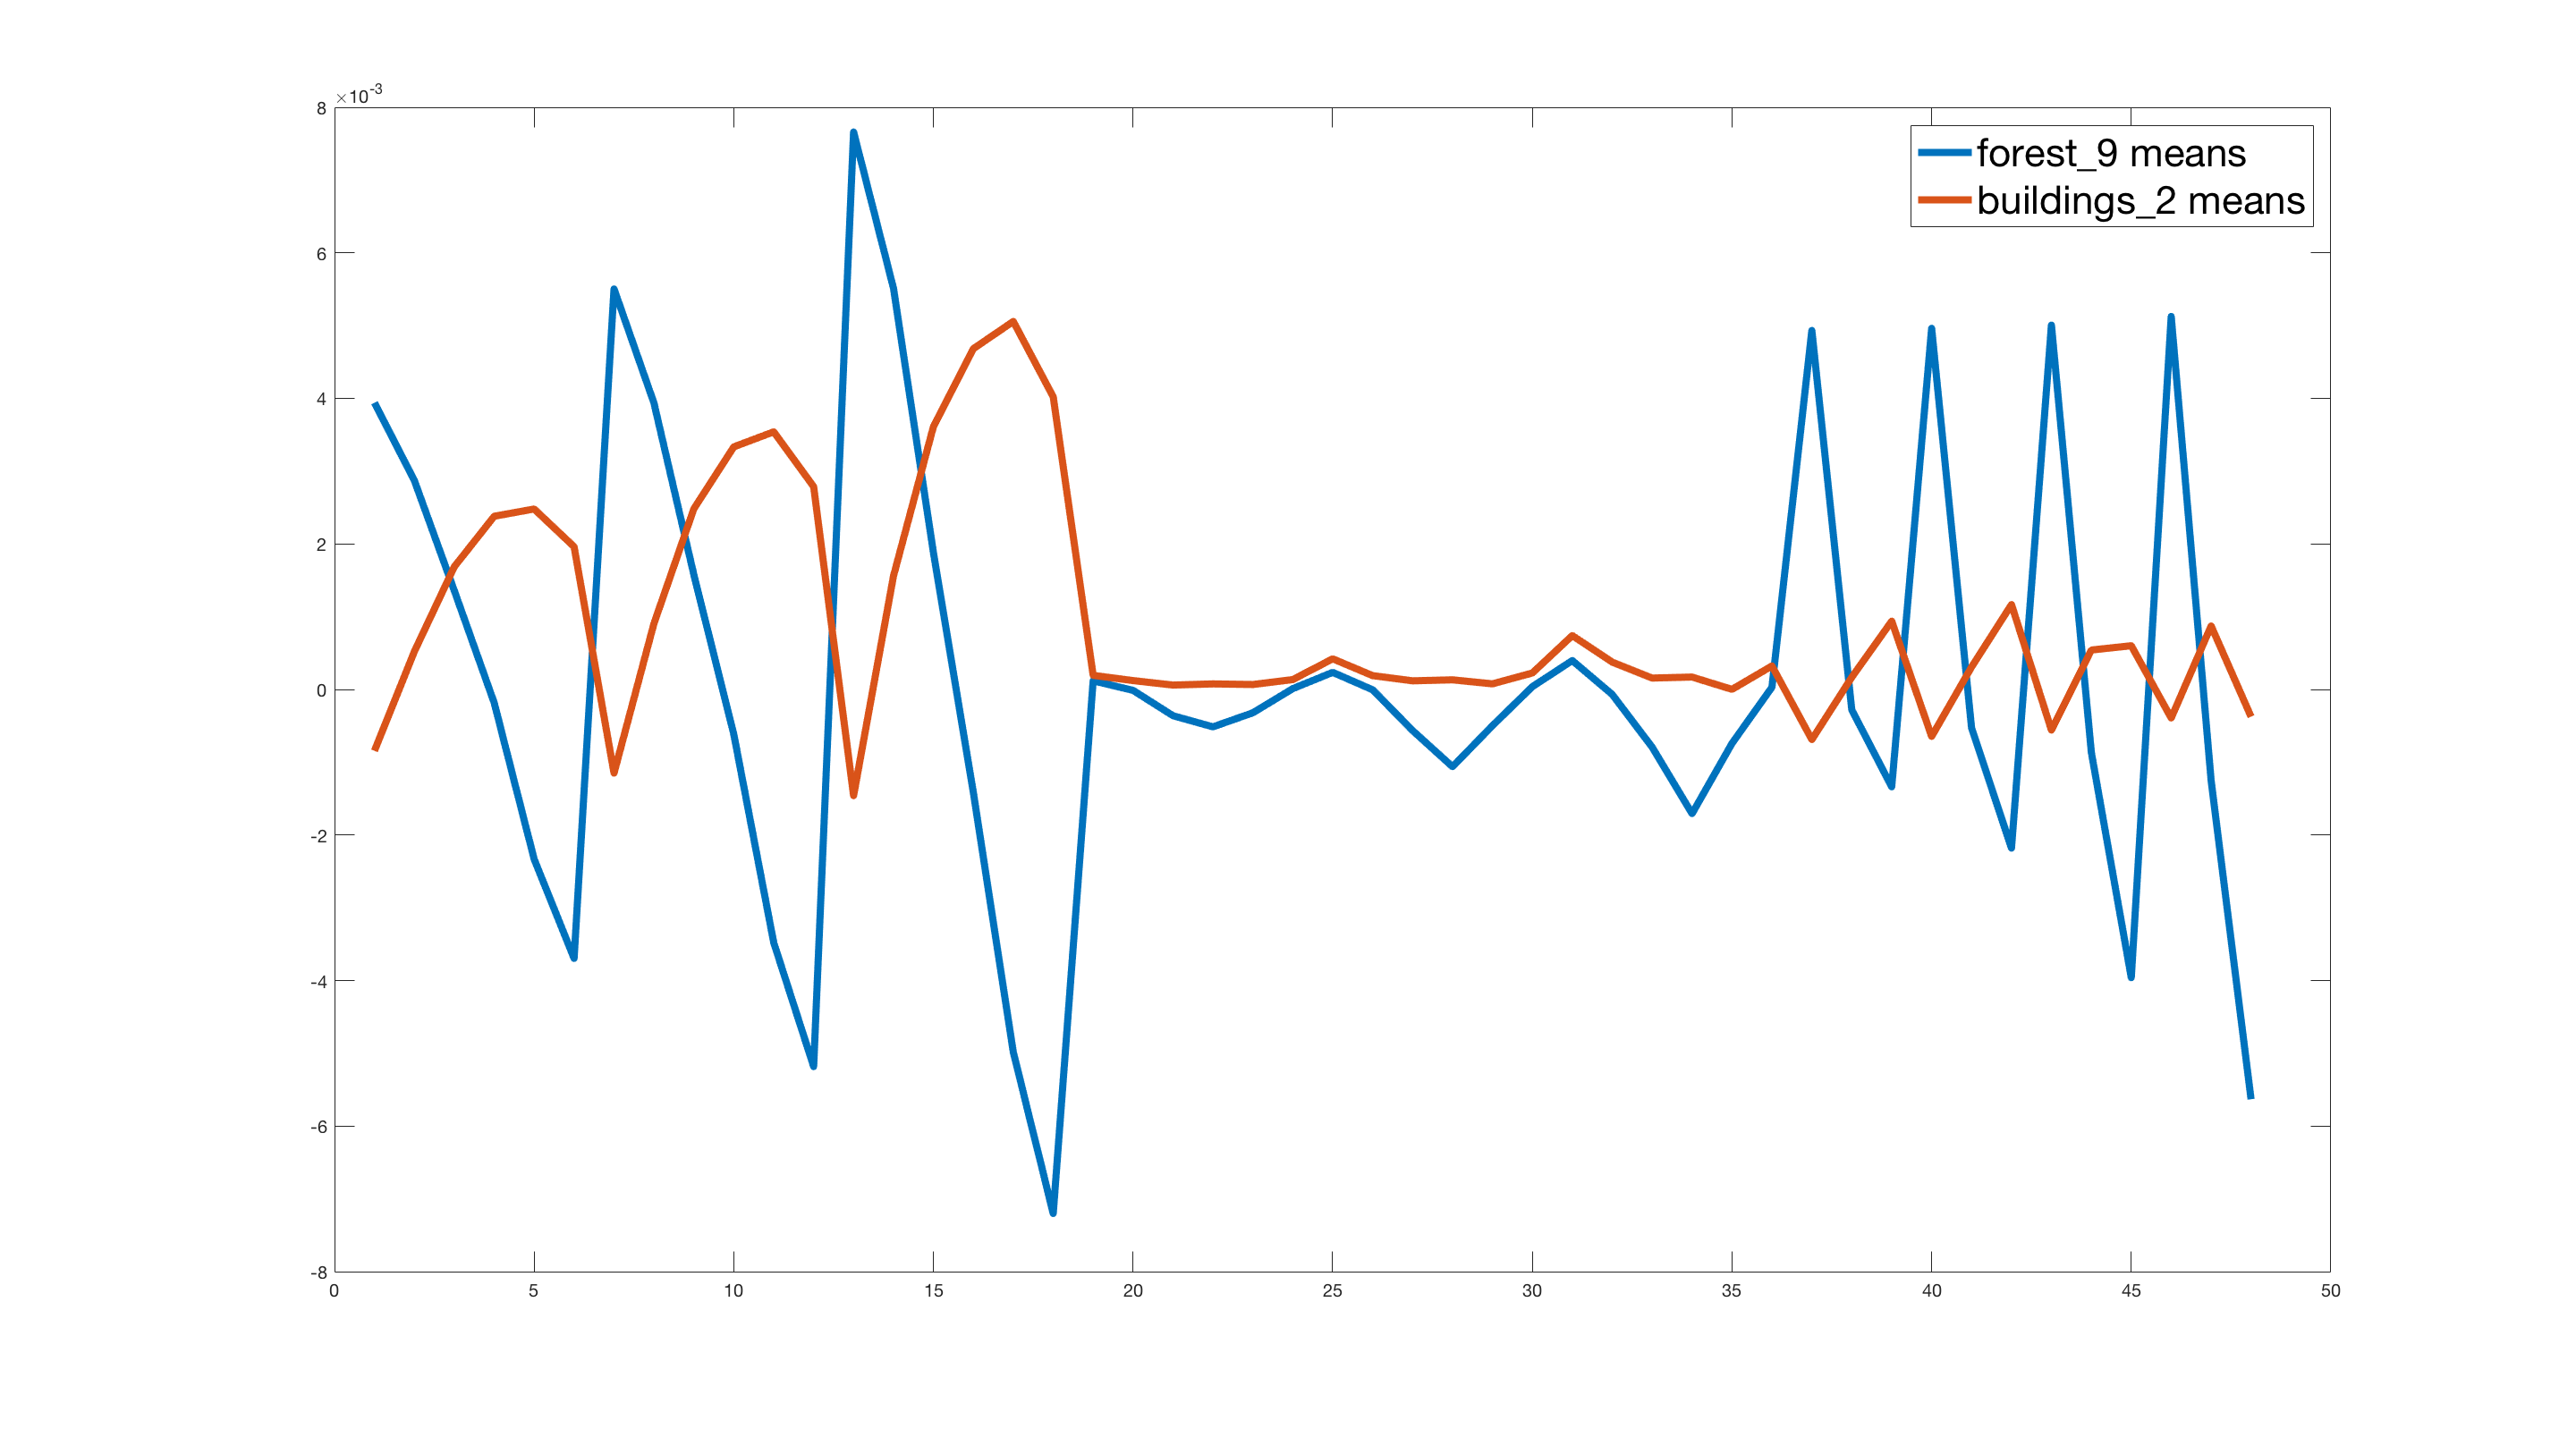
\includegraphics[width=0.45\textwidth]{img/f9b2_means}}
\subfigure[test]{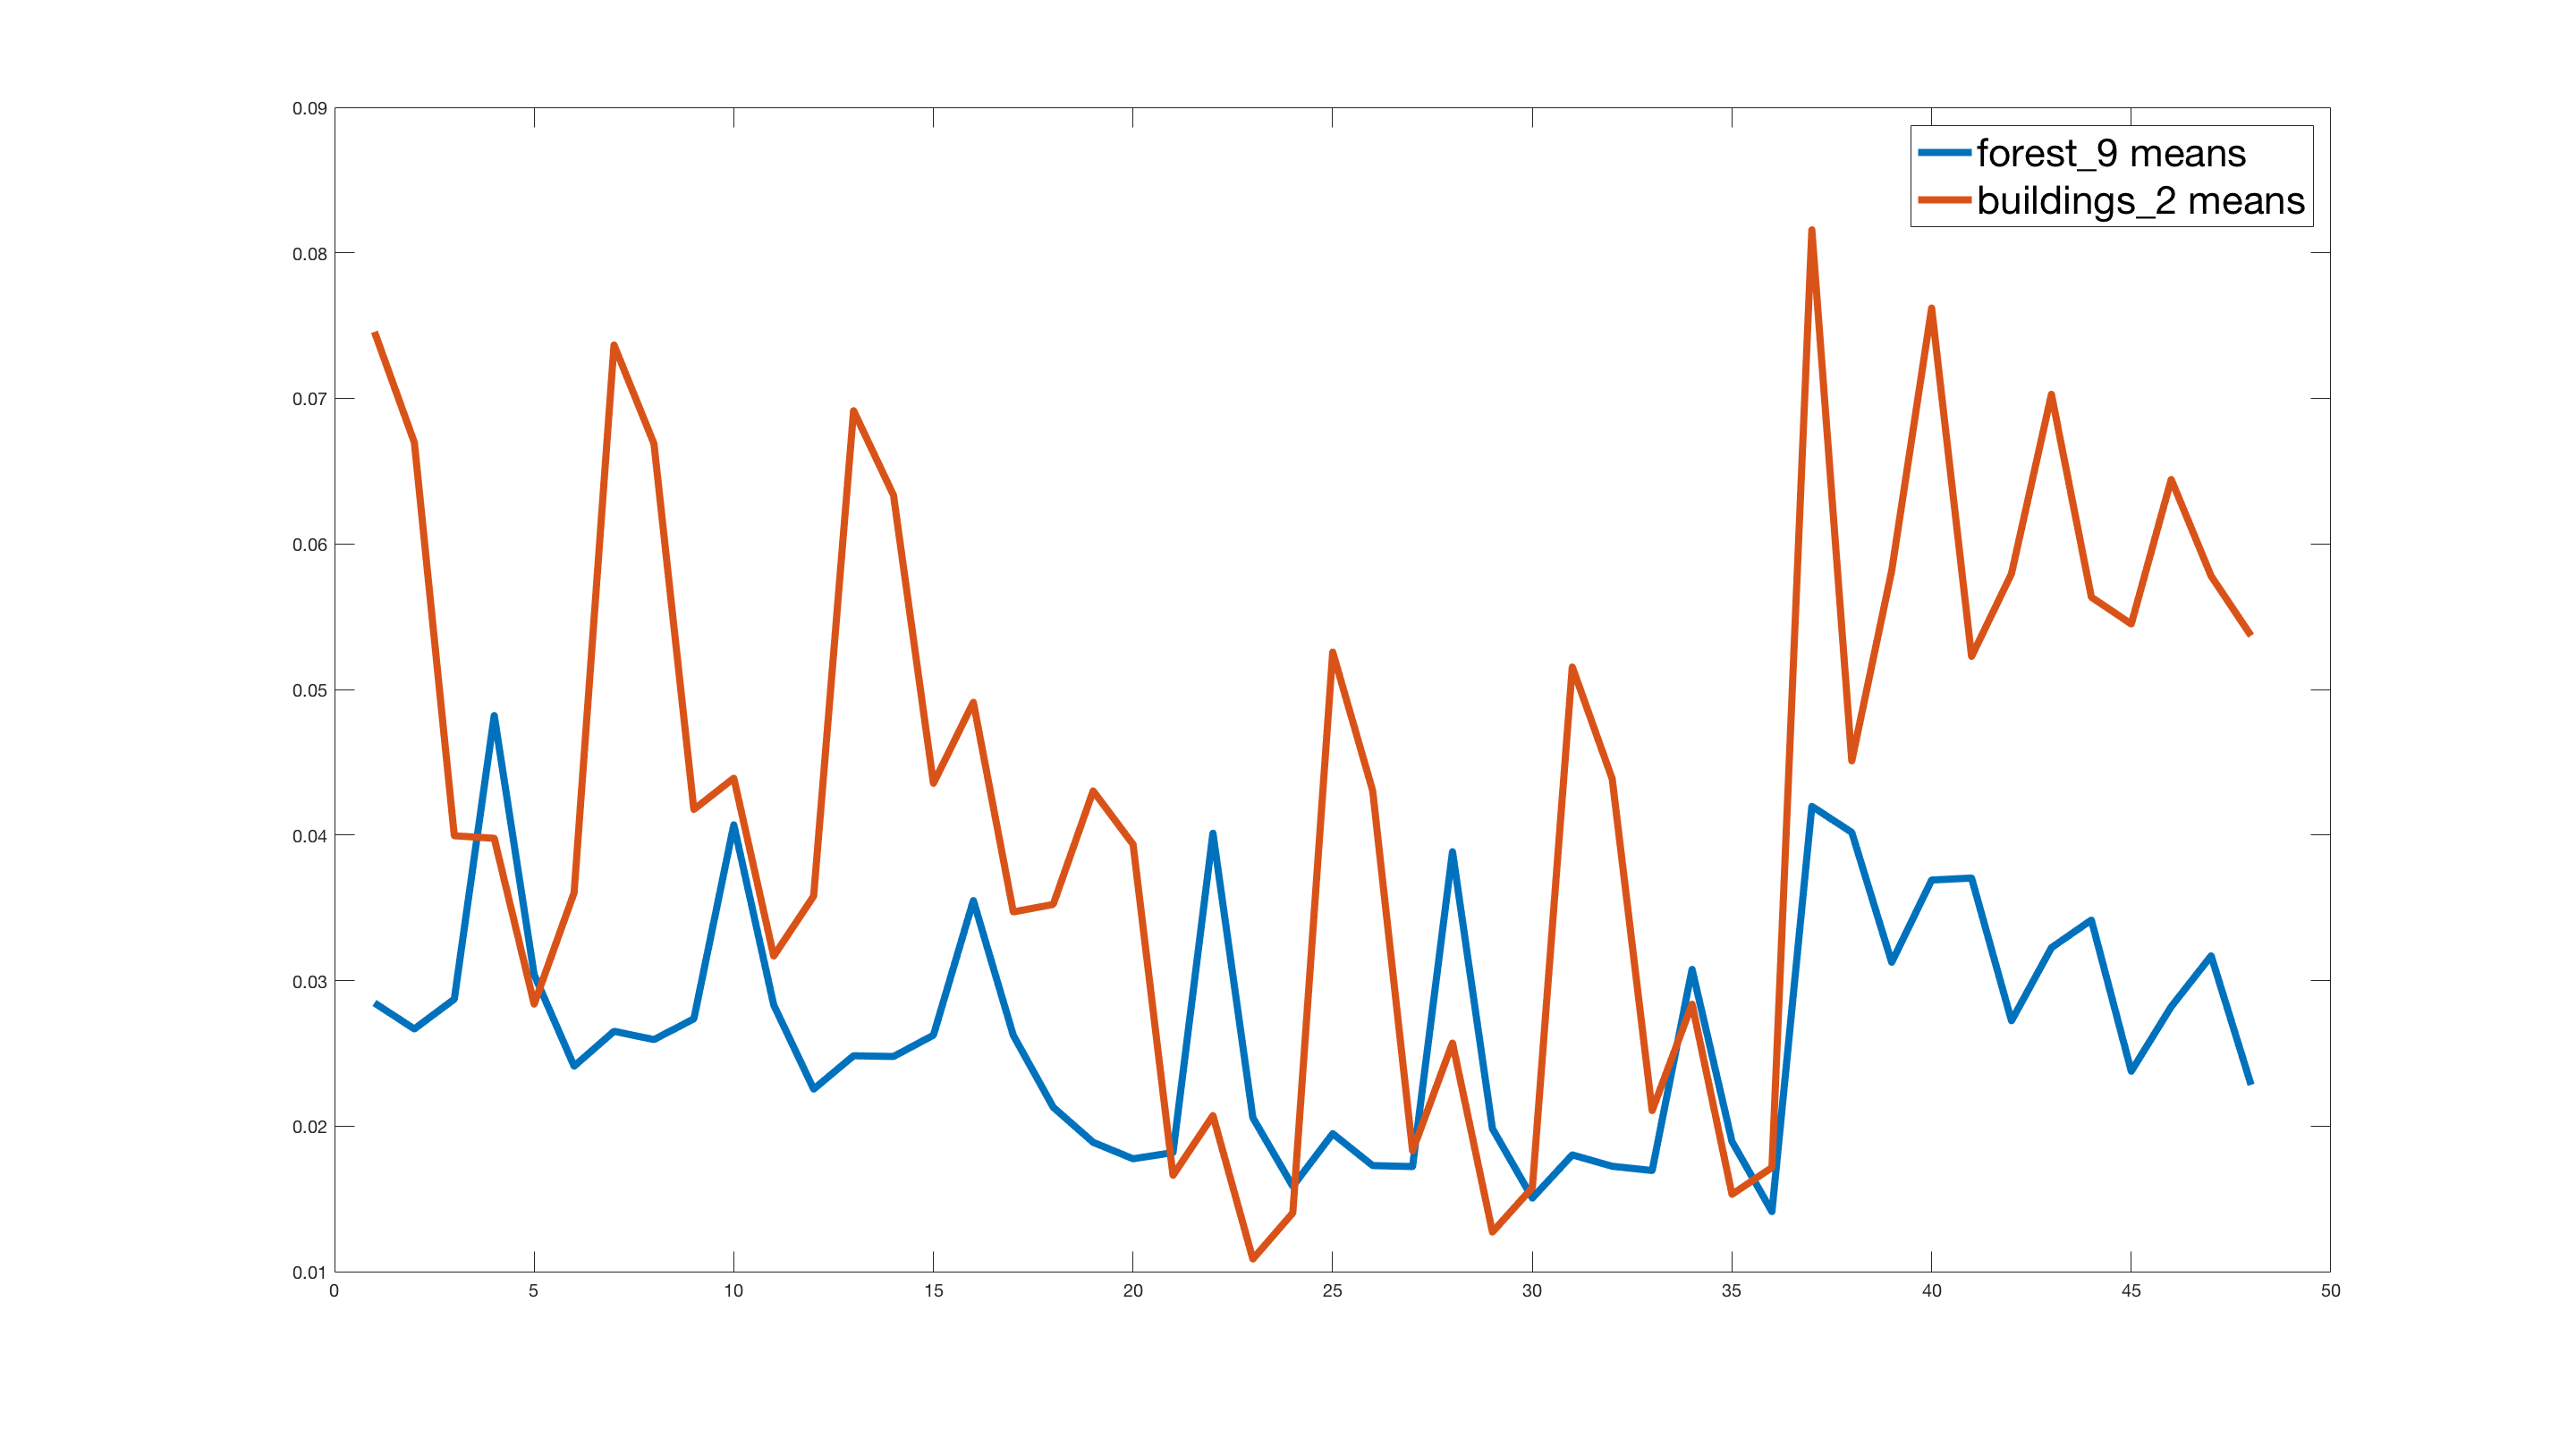
\includegraphics[width=0.45\textwidth]{img/f9b2_sds}}
\caption{cap}
\label{fig:means}
\end{figure}

\section{Class Feature Matrices}

When applying the convolutions of the LM filter bank, responses for the filters are usually different in different parts of an image. In order to describe an image's texture with a small but expressive number of descriptors, we need to aggregate the responses of the image for each filter into single values. For this we can calculate descriptive metrics such as mean, standard deviation, or median. We construct a feature matrix for each class (forest, buildings, and sunset) of images with each row corresponding to an image and each column corresponding to the aggregated response of this image to a filter of the LM filter bank.

\section{Visualizing Class Feature Differences}

\begin{figure}[!hbt]
  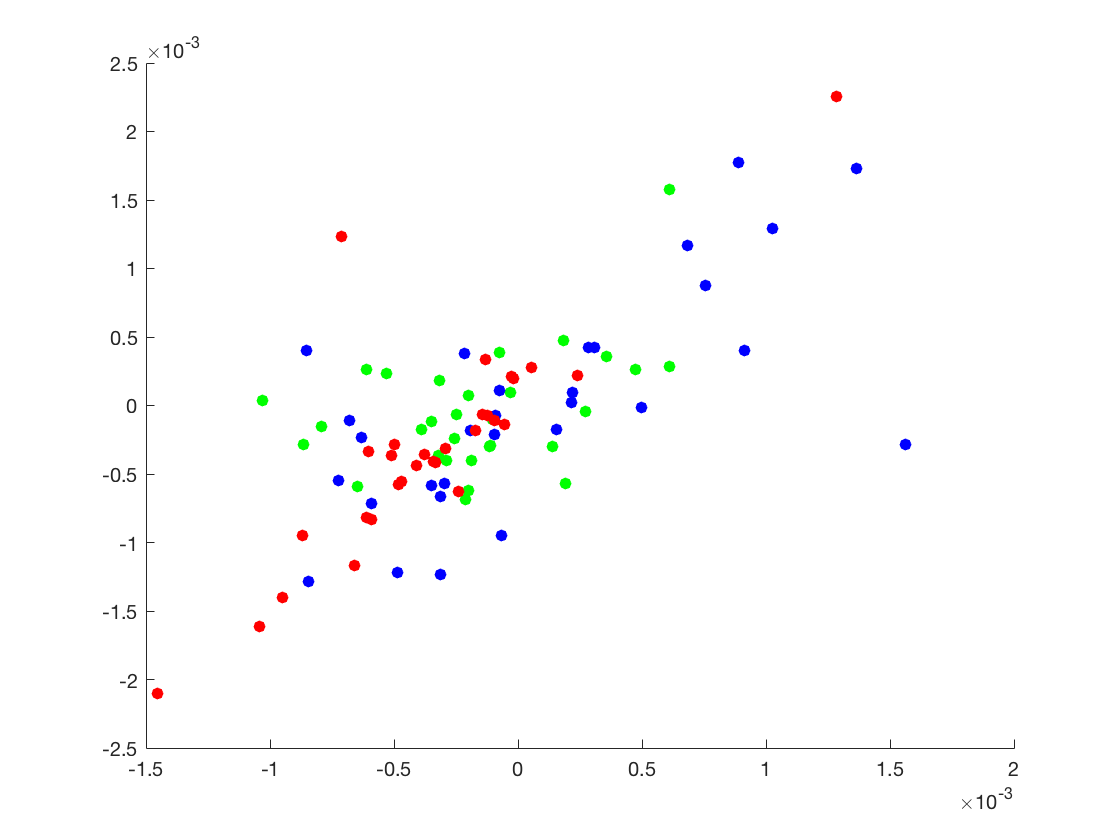
\includegraphics[width=\textwidth]{img/m41_m25}
    \caption{test}
  \label{fig:m41_m25}
\end{figure}

\begin{figure}[!hbt]
  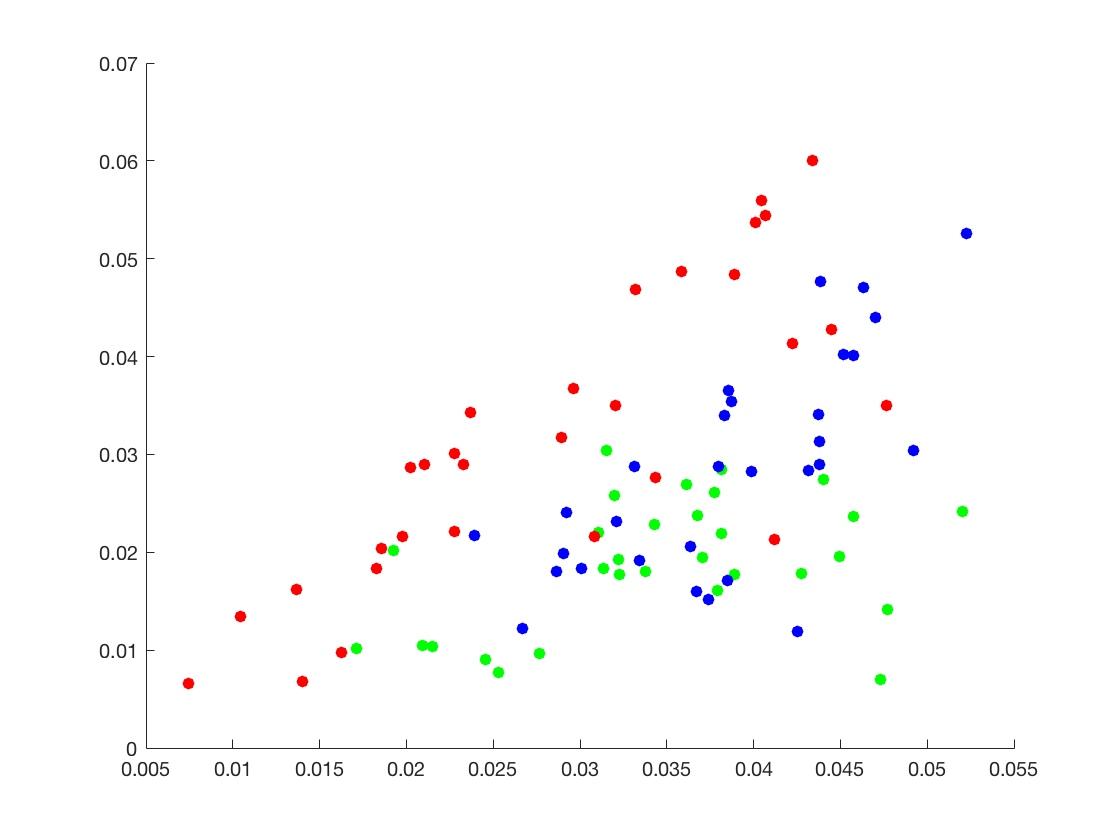
\includegraphics[width=\textwidth]{img/sd41_sd25}
    \caption{test}
  \label{fig:sd41_sd25}
\end{figure}

\begin{figure}[!hbt]
  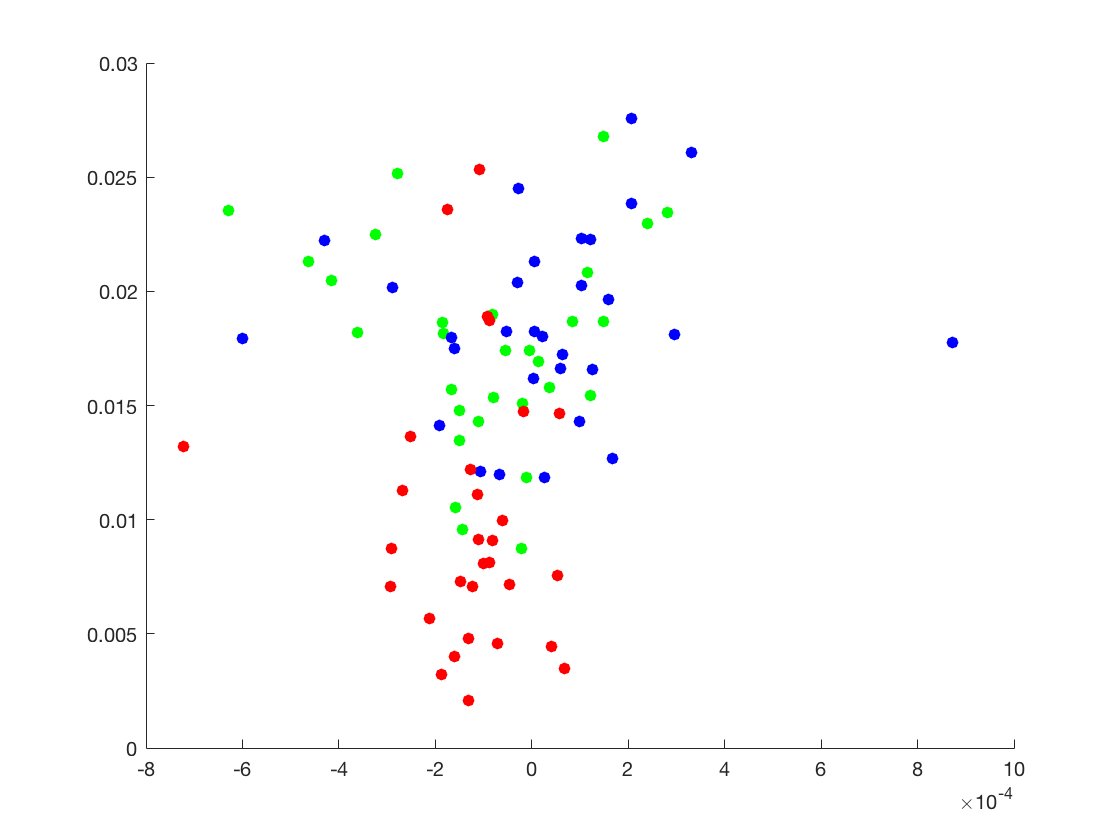
\includegraphics[width=\textwidth]{img/m21_sd21}
    \caption{test}
  \label{fig:m21_sd21}
\end{figure}

\section{KNN Search for Similar Images}


\begin{figure}[!hbt]
\centering
\subfigure[test]{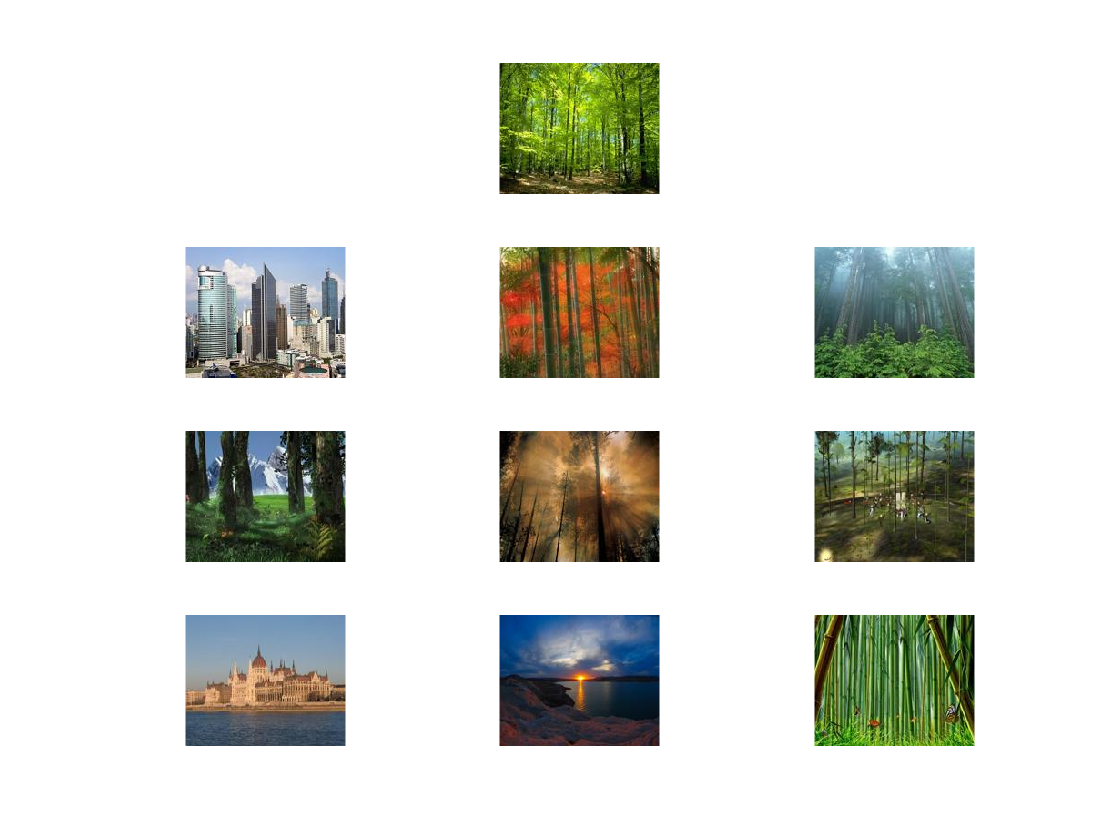
\includegraphics[width=0.45\textwidth]{img/f9knn_100000}}
\subfigure[test]{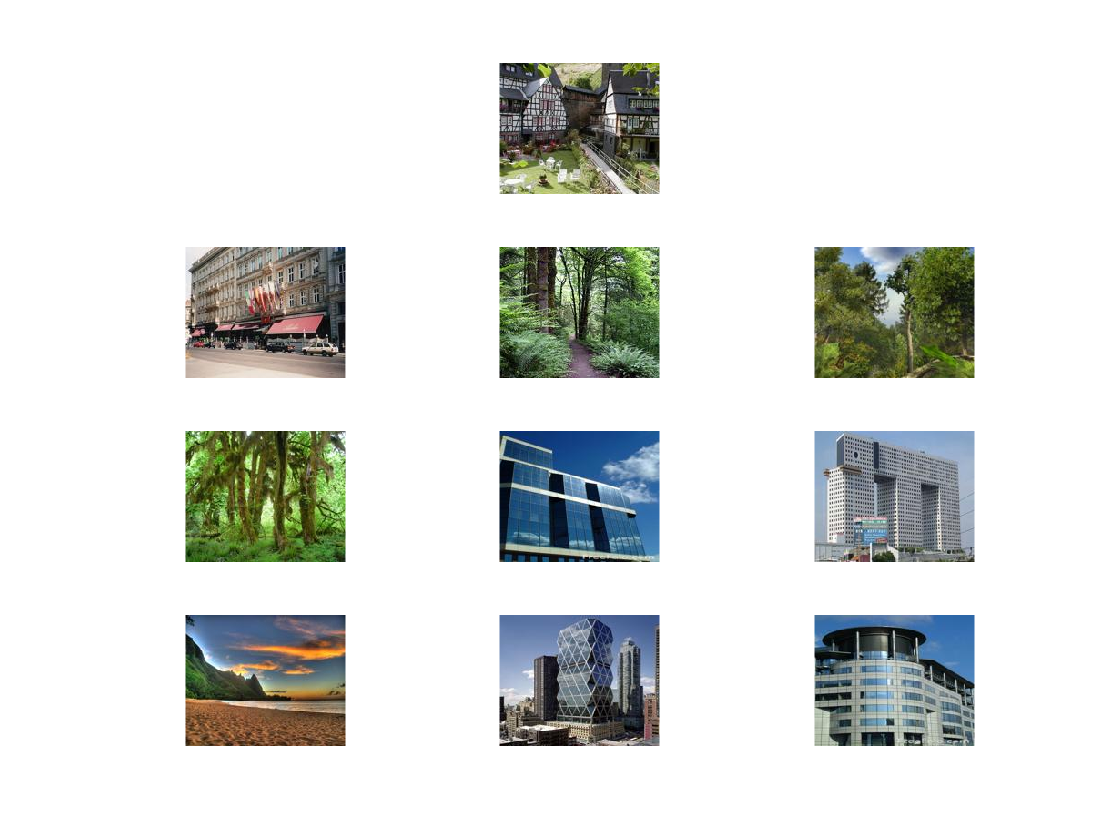
\includegraphics[width=0.45\textwidth]{img/b5knn_100000}}
\caption{cap 100000}
\label{fig:100000}
\end{figure}

\begin{figure}[!hbt]
\centering
\subfigure[test]{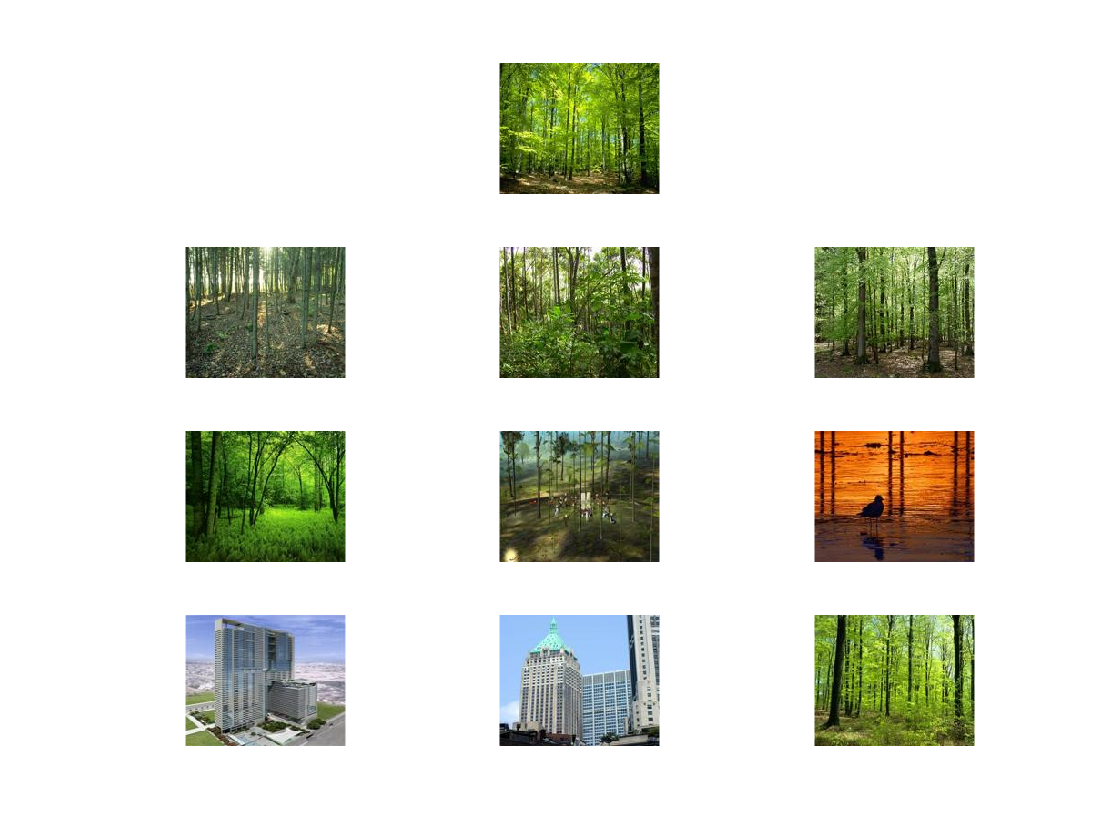
\includegraphics[width=0.45\textwidth]{img/f9knn_010000}}
\subfigure[test]{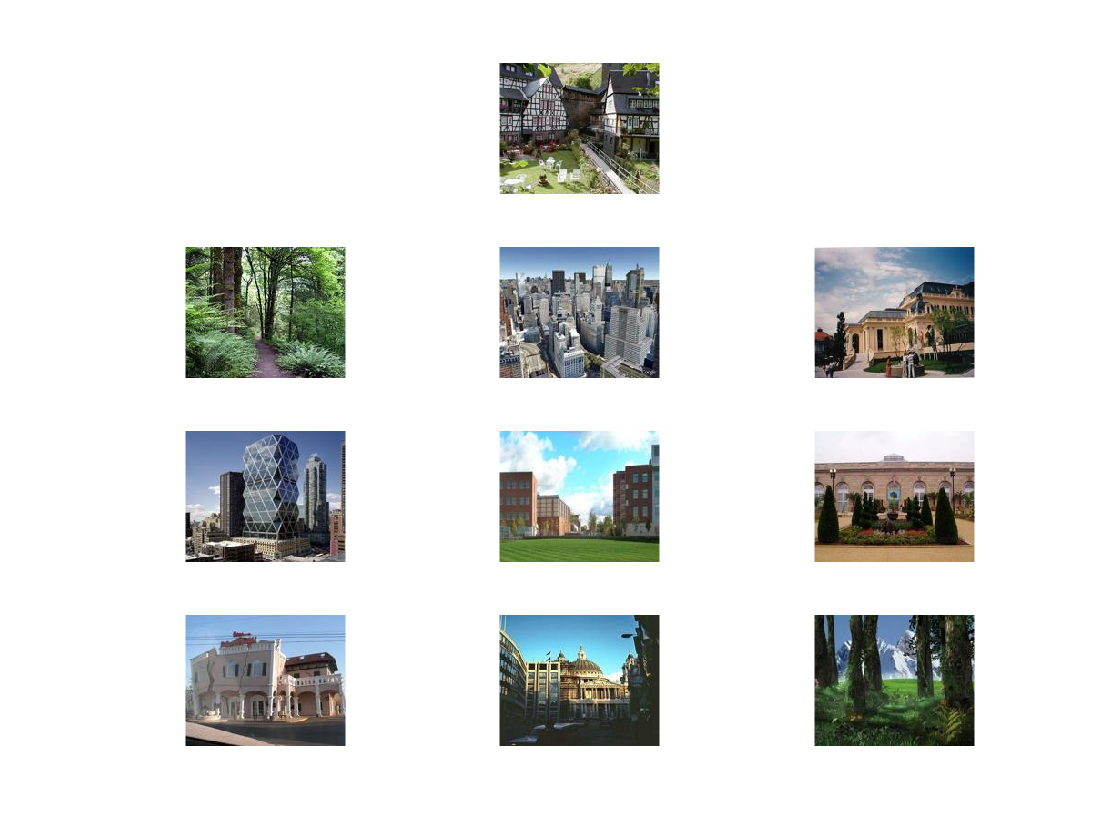
\includegraphics[width=0.45\textwidth]{img/b5knn_010000}}
\caption{cap 010000}
\label{fig:010000}
\end{figure}

\begin{figure}[!hbt]
\centering
\subfigure[test]{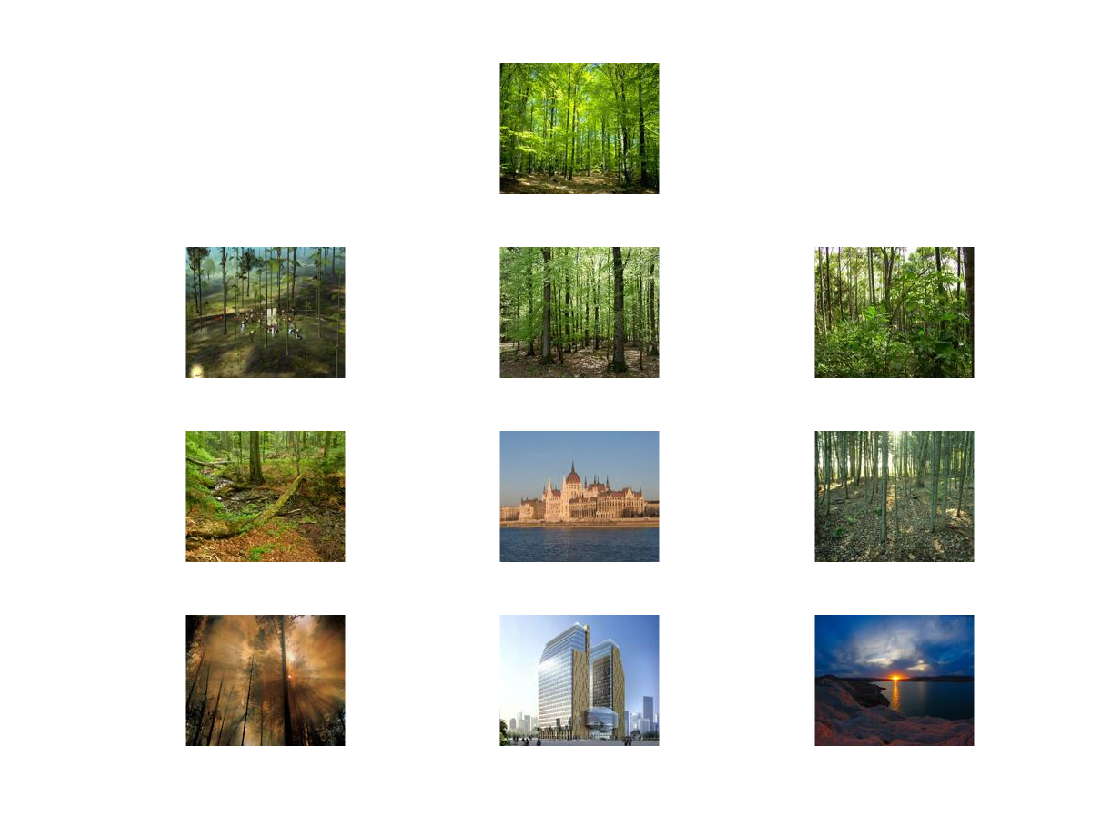
\includegraphics[width=0.45\textwidth]{img/f9knn_111110}}
\subfigure[test]{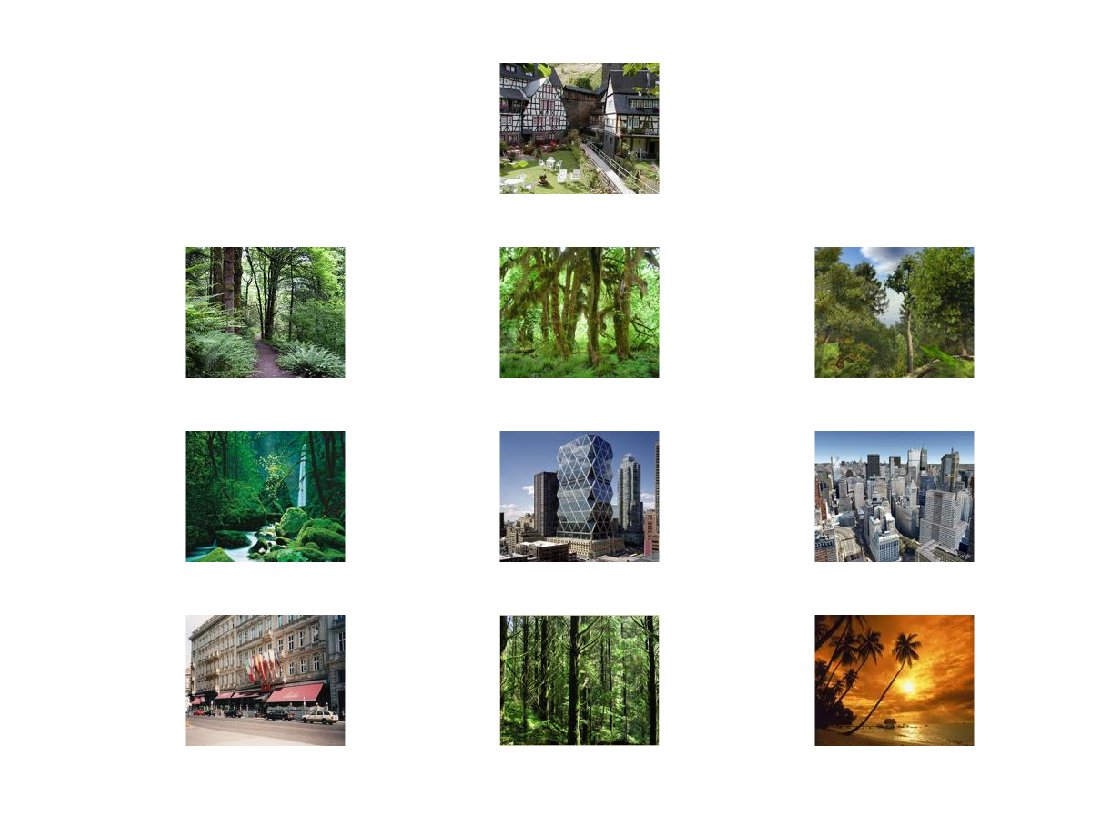
\includegraphics[width=0.45\textwidth]{img/b5knn_111110}}
\caption{cap 111110}
\label{fig:111110}
\end{figure}

looking at the separability of color:


\begin{figure}[!hbt]
\centering
\subfigure[test]{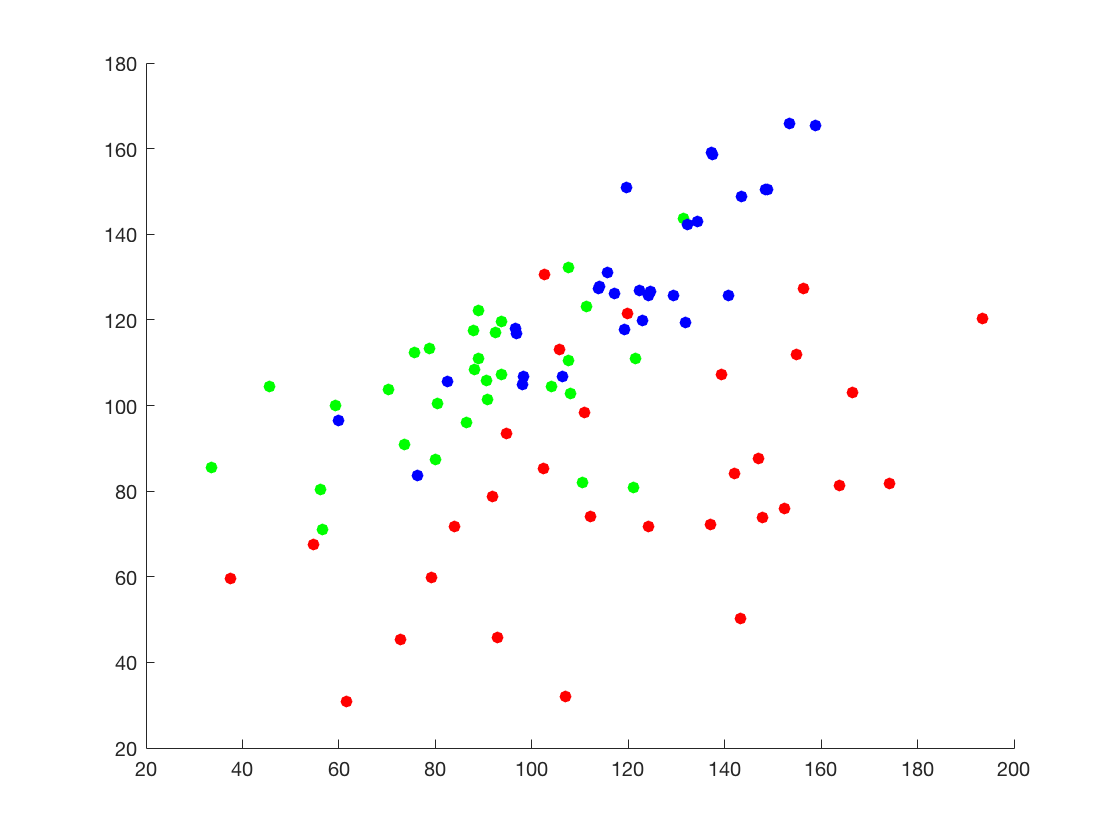
\includegraphics[width=0.33\textwidth]{img/mr_mg}}
\subfigure[test]{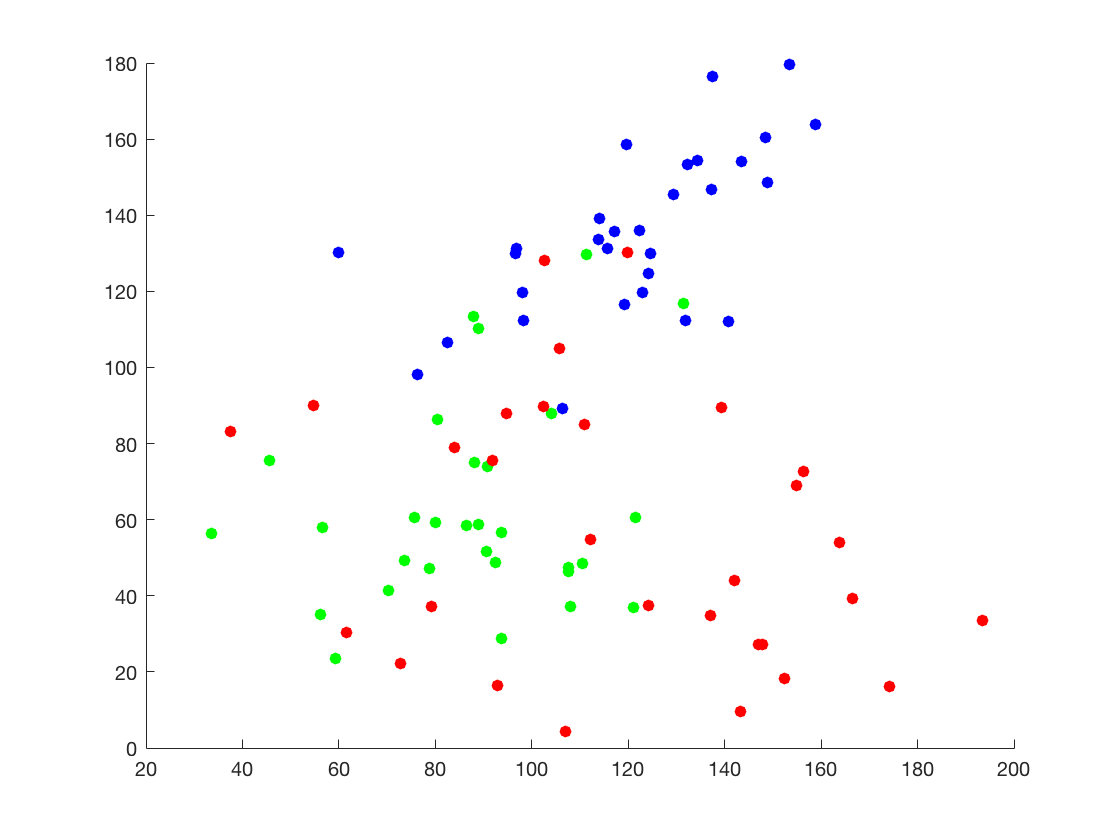
\includegraphics[width=0.33\textwidth]{img/mr_mb}}
\subfigure[test]{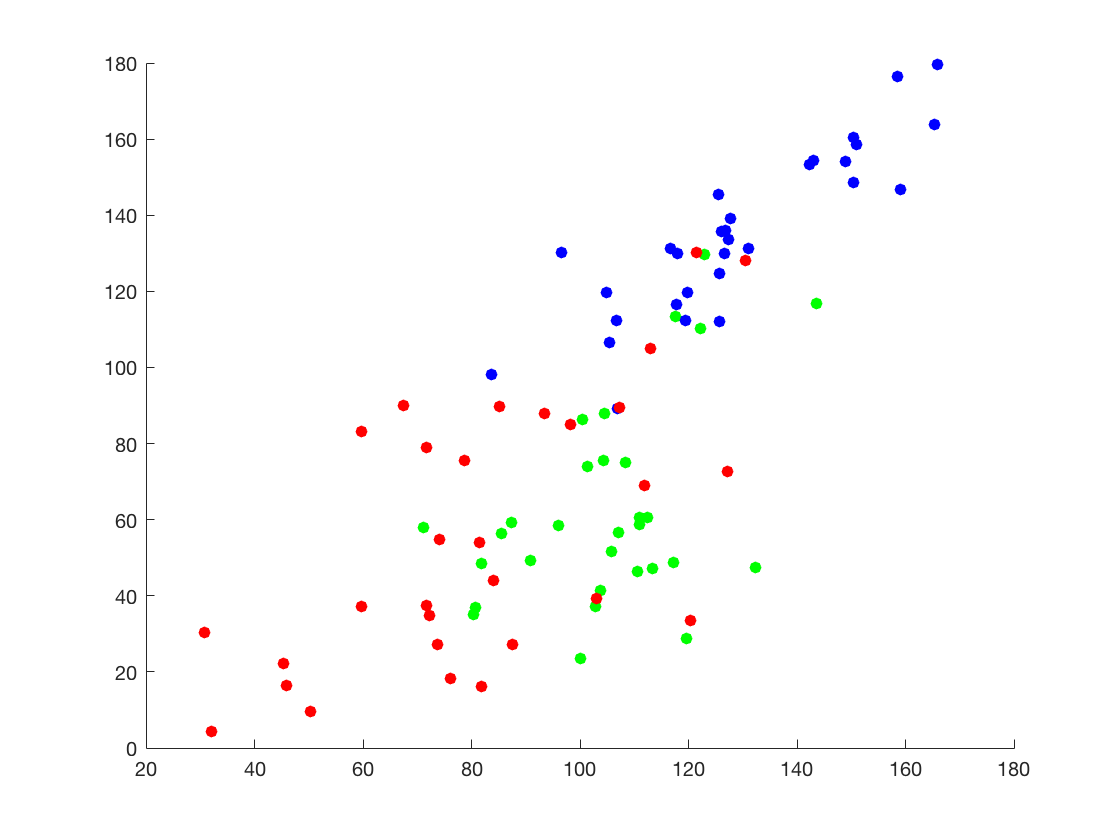
\includegraphics[width=0.33\textwidth]{img/mb_mg}}
\caption{Separability of RGB features}
\label{fig:mrgb}
\end{figure}

\begin{figure}[!hbt]
\centering
\subfigure[test]{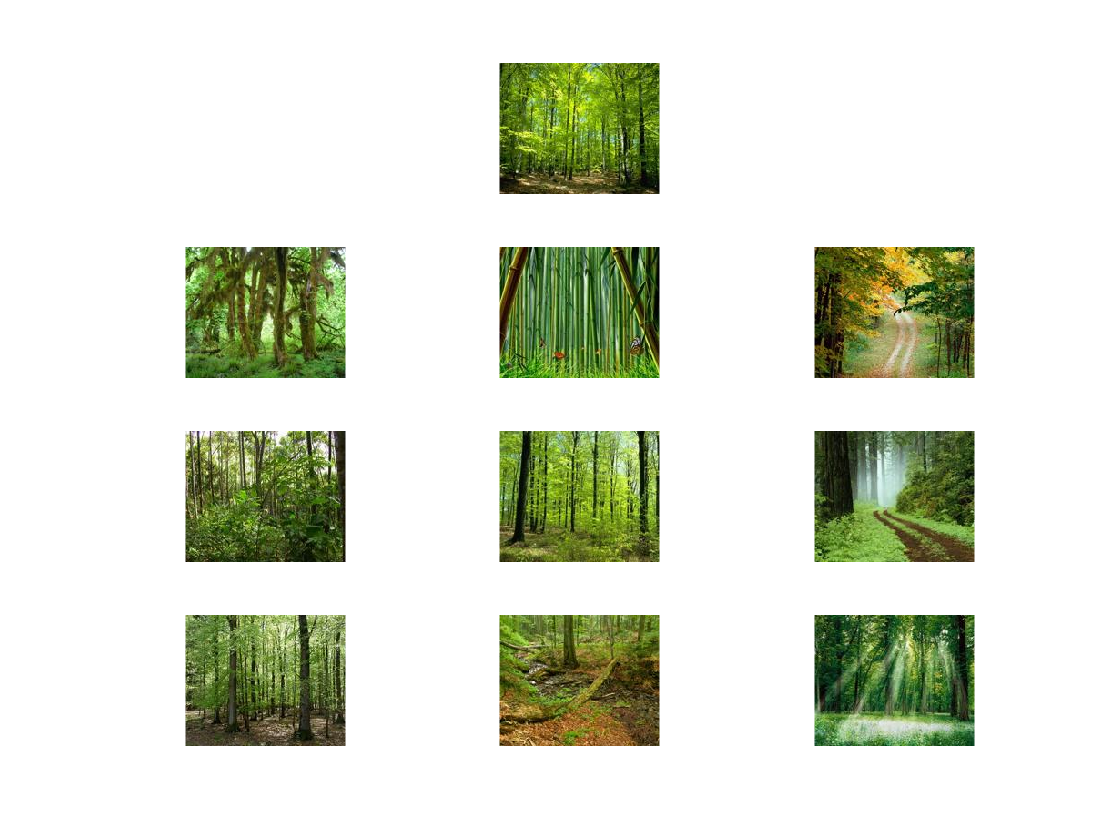
\includegraphics[width=0.45\textwidth]{img/f9knn_000001}}
\subfigure[test]{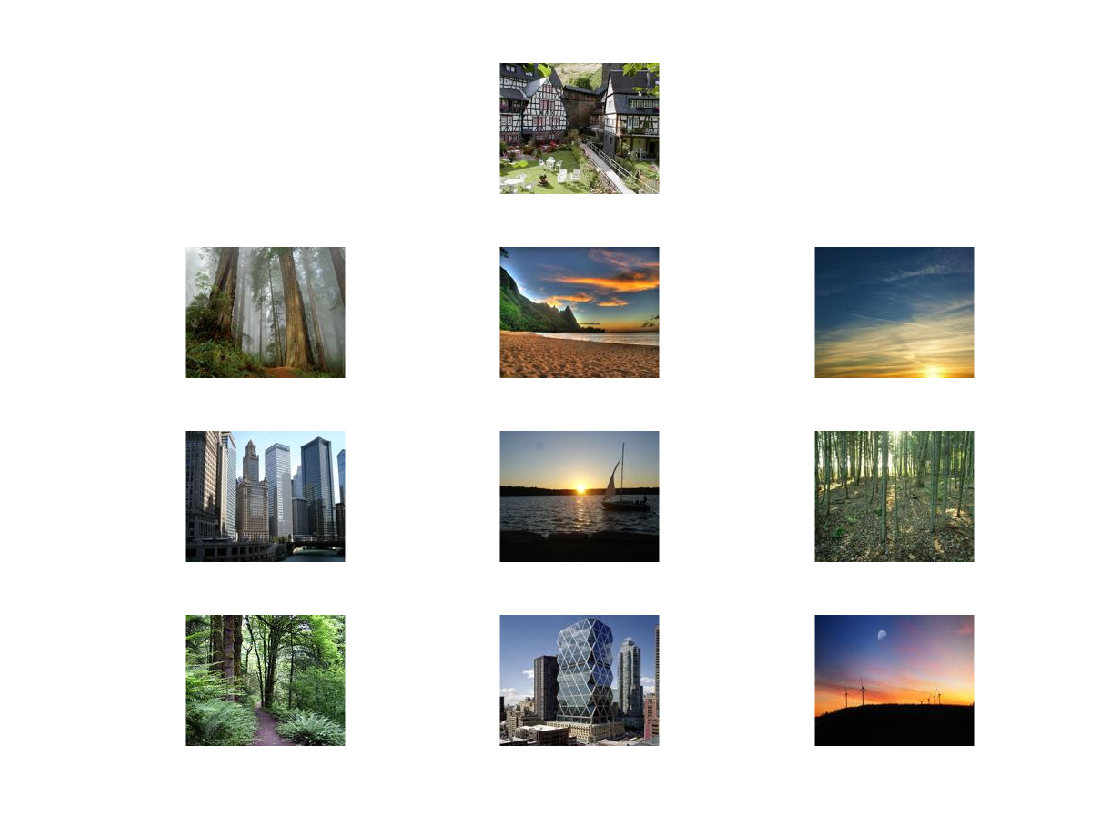
\includegraphics[width=0.45\textwidth]{img/b5knn_000001}}
\caption{cap 000001}
\label{fig:000001}
\end{figure}

\begin{figure}[!hbt]
\centering
\subfigure[test]{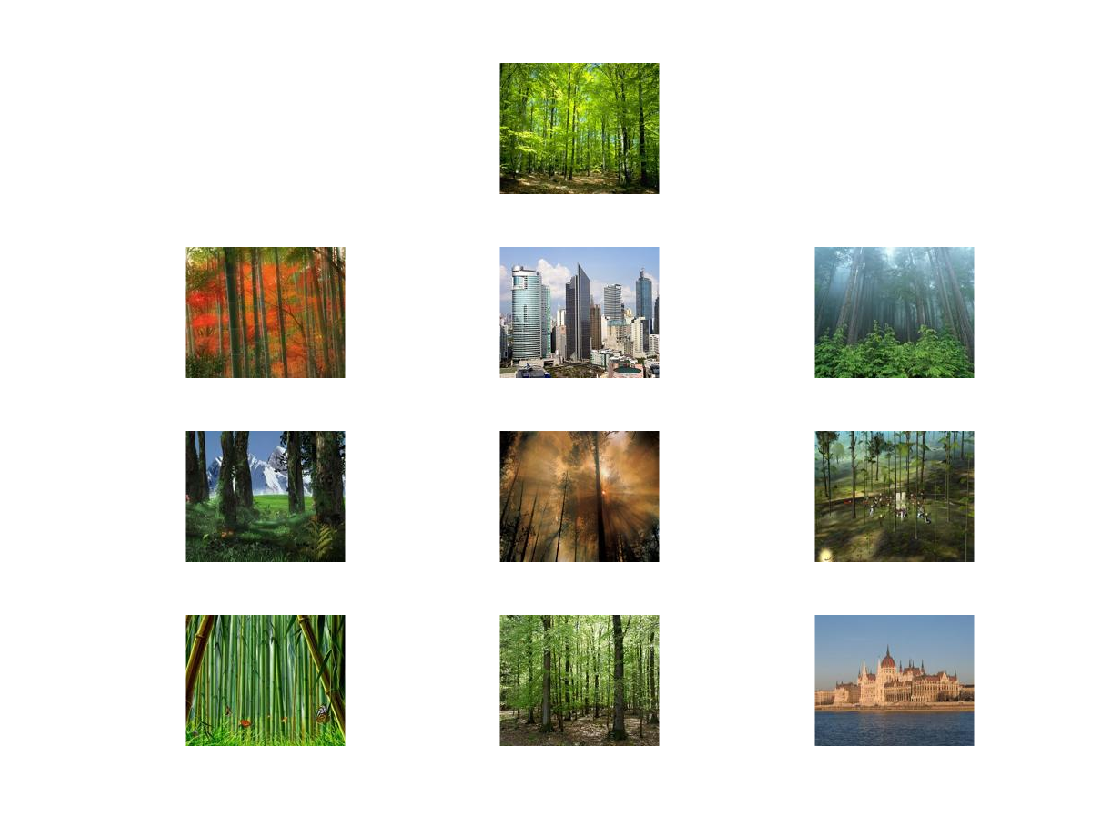
\includegraphics[width=0.45\textwidth]{img/f9knn_100001}}
\subfigure[test]{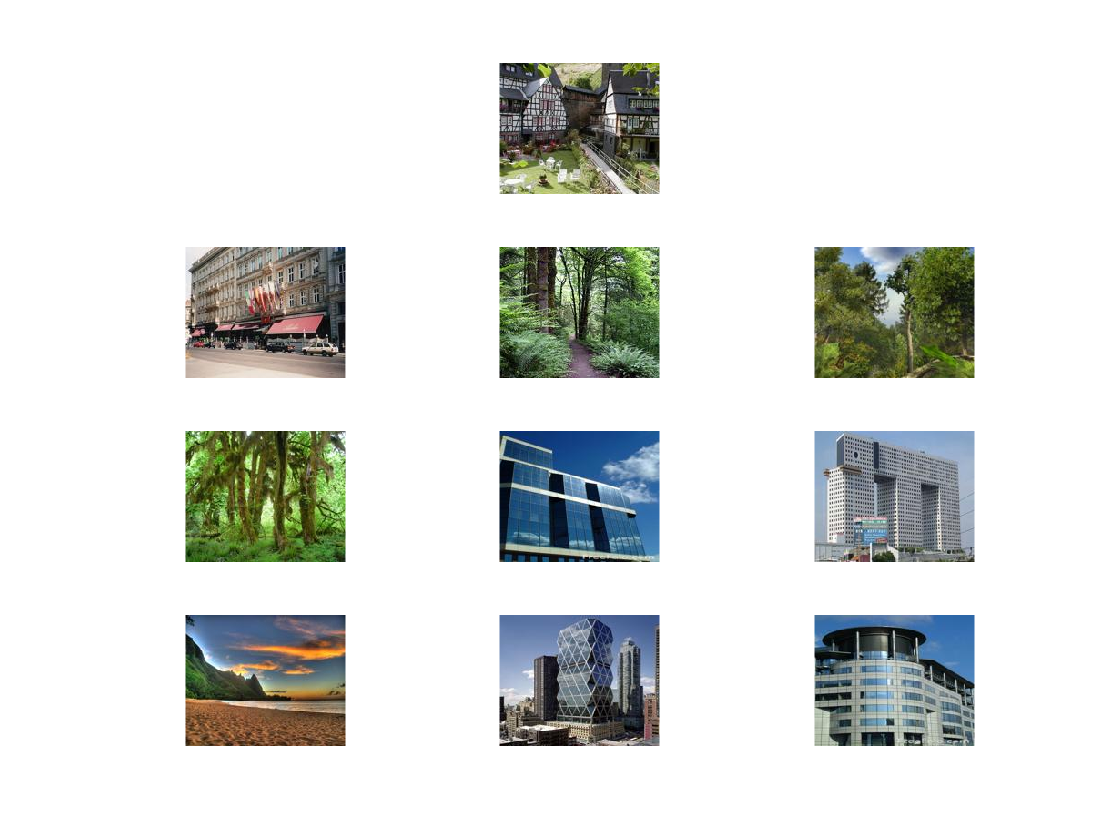
\includegraphics[width=0.45\textwidth]{img/b5knn_100001}}
\caption{cap 100001}
\label{fig:100001}
\end{figure}

\begin{figure}[!hbt]
\centering
\subfigure[test]{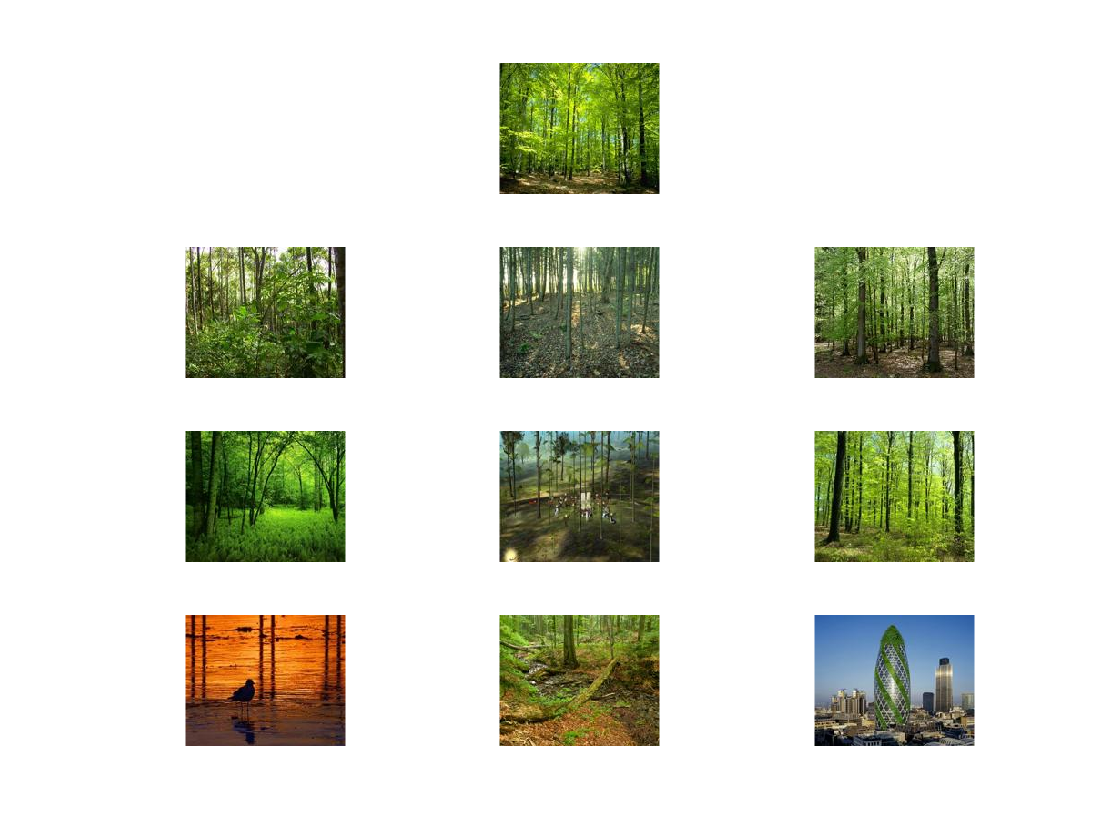
\includegraphics[width=0.45\textwidth]{img/f9knn_010001}}
\subfigure[test]{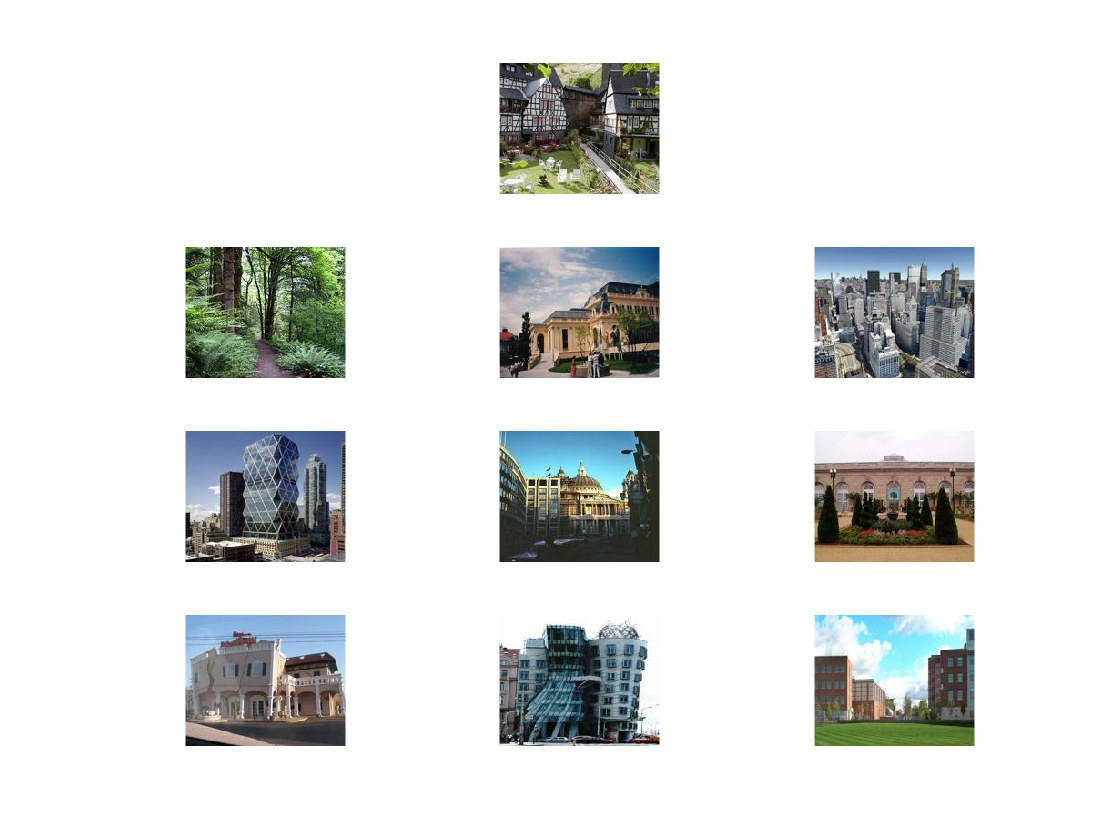
\includegraphics[width=0.45\textwidth]{img/b5knn_010001}}
\caption{cap 010001}
\label{fig:010001}
\end{figure}

featureModes =

     1     0     0     0     0     0


ans =

    0.4222


featureModes =

     0     1     0     0     0     0


ans =

    0.6333


featureModes =

     0     0     1     0     0     0


ans =

    0.5778


featureModes =

     0     0     0     1     0     0


ans =

    0.5333


featureModes =

     0     0     0     0     1     0


ans =

    0.4000


featureModes =

     0     0     0     0     0     1


ans =

    0.7556

featureModes =

     1     0     0     0     0     1


ans =

    0.5333


featureModes =

     0     1     0     0     0     1


ans =

    0.7111


featureModes =

     0     0     1     0     0     1


ans =

    0.5889


featureModes =

     0     0     0     1     0     1


ans =

    0.6889


featureModes =

     0     0     0     0     1     1


ans =

    0.5000


featureModes =

     1     1     1     1     1     0


ans =

    0.4556


featureModes =

     1     1     1     1     1     1


ans =

    0.5111